\documentclass[10pt,journal,compsoc]{IEEEtran}
% Load basic packages
\usepackage{balance}  % to better equalize the last page
\usepackage{graphics} % for EPS, load graphicx instead 
\usepackage[T1]{fontenc}
% \usepackage{txfonts}
% \usepackage{mathptmx}
\usepackage[pdftex]{hyperref}
\usepackage{color}
\usepackage{xcolor}
\usepackage{booktabs}
\usepackage{textcomp}
\usepackage{xspace}
\usepackage{setspace}
\usepackage[textsize=tiny]{todonotes}
% Some optional stuff you might like/need.
\usepackage{microtype} % Improved Tracking and Kerning
% \usepackage[all]{hypcap}  % Fixes bug in hyperref caption linking
\usepackage{ccicons}  % Cite your images correctly!
% \usepackage[utf8]{inputenc} % for a UTF8 editor only
\usepackage{verbatim}
\usepackage{relsize}
\usepackage{etoolbox}
\usepackage{lipsum}   % for filler text
\usepackage{setspace} % for \onehalfspacing and \singlespacing macros
\usepackage[normalem]{ulem}
\usepackage[sort,nocompress]{cite}
\usepackage{xcolor}
\usepackage{fixltx2e}
\usepackage{amsmath}
\usepackage{amssymb}
\usepackage{afterpage}
\usepackage{microtype}                 % use micro-typography (slightly more compact, better to read)
\PassOptionsToPackage{warn}{textcomp}  % to address font issues with \textrightarrow
\usepackage{times}                     % we use Times as the main font
\renewcommand*\ttdefault{txtt}         % a nicer typewriter font
\usepackage{cite}                      % needed to automatically sort the references
\usepackage{tabu}                      % only used for the table example
\usepackage{booktabs}                  % only used for the table example
\usepackage{amsmath}
\usepackage[linesnumbered,ruled]{algorithm2e}
\usepackage{tikz}
\usetikzlibrary{shapes,arrows}

\DeclareMathOperator*{\argmax}{arg\,max}
% llt: Define a global style for URLs, rather that the default one
\makeatletter
\def\url@leostyle{%
  \@ifundefined{selectfont}{
    \def\UrlFont{\sf}
  }{
    \def\UrlFont{\small\bf\ttfamily}
  }}
\makeatother

\newenvironment{denselist}{
    \begin{list}{\small{$\bullet$}}%
    {\setlength{\itemsep}{0ex} \setlength{\topsep}{0ex}
    \setlength{\parsep}{0pt} \setlength{\itemindent}{0pt}
    \setlength{\leftmargin}{1.5em}
    \setlength{\partopsep}{0pt}}}%
    {\end{list}}

\newcommand{\squishlist}{
   \begin{list}{$\bullet$}
    { \setlength{\itemsep}{0pt}
      \setlength{\parsep}{2pt}
      \setlength{\topsep}{0pt}
      \setlength{\partopsep}{0pt}
      \leftmargin=25pt
\rightmargin=0pt
\labelsep=5pt
\labelwidth=10pt
\itemindent=0pt
\listparindent=0pt
\itemsep=\parsep
    }
}
\newcommand{\squishend}{\end{list}}
\newcommand{\npar}{\par \noindent}
% use extensively to toggle between paper and TR
\newcommand{\eat}[1]{}
% \newcommand{\papertext}[1]{{\leavevmode\color{blue}{#1}}}
% \newcommand{\techreport}[1]{{\leavevmode\color{red}{#1}}}
\newcommand{\papertext}[1]{#1}
\newcommand{\techreport}[1]{}
\newcommand{\boldpara}[1]{\textbf{\paragraph{#1}}}
% de-facto paragraph format
\newcommand{\stitle}[1]{\noindent\textbf{#1}}
\newcommand{\tvcg}[1]{{\leavevmode\color{blue}{#1}}}
\newcommand{\cut}[1]{{\leavevmode\color{lightgray}{#1}}}
\newcommand{\ccut}[1]{} %confirmed cut
\newcommand{\system}{\textsc{Storyboard}\xspace}
\def\plaintitle{\system : Hierarchical Summary of Equivalent Visualizations across Data Subsets}
\def\plainauthor{Doris Jung-Lin Lee*, Himel Dev*, Huizi Hu, Hazem Elmeleegy, Aditya Parameswaran}
\def\emptyauthor{} 
\def\plainkeywords{Data visualization, exploratory data analysis, visual query, scientific data.}
\def\plaingeneralterms{Documentation, Standardization}

\newcommand{\agp}[1]{\textcolor{blue}{Aditya: #1}}
\newcommand{\dor}[1]{\textcolor{green}{Doris: #1}} 
\newcommand{\hdev}[1]{\textcolor{magenta}{Himel: #1}}
\newcommand{\haz}[1]{\textcolor{orange}{Hazem: #1}}
\newcommand\notes[1]{\textcolor{red}{#1}}
\urlstyle{leo}

% To make various LaTeX processors do the right thing with page size.
\def\pprw{8.5in}
\def\pprh{11in}
\special{papersize=\pprw,\pprh}
\setlength{\paperwidth}{\pprw}
\setlength{\paperheight}{\pprh}
\setlength{\pdfpagewidth}{\pprw}
\setlength{\pdfpageheight}{\pprh}

% Make sure hyperref comes last of your loaded packages, to give it a
% fighting chance of not being over-written, since its job is to
% redefine many LaTeX commands.
\definecolor{linkColor}{RGB}{6,125,233}
\hypersetup{%
  pdftitle={\plaintitle},
% Use \plainauthor for final version.
%  pdfauthor={\plainauthor},
  pdfauthor={\emptyauthor},
  pdfkeywords={\plainkeywords},
  bookmarksnumbered,
  pdfstartview={FitH},
  colorlinks,
  citecolor=black,
  filecolor=black,
  linkcolor=black,
  urlcolor=linkColor,
  breaklinks=true}


% Get rid of gaps between sections, subsections and subsubsections
% \usepackage{titlesec}
% \titlespacing*{\section}
% {0pt}{0pt}{0pt}
% \titlespacing*{\subsection}
% {0pt}{0pt}{0pt}
% \titlespacing*{\subsubsection}
% {0pt}{0pt}{0pt}
% End of preamble. Here it comes the document.

\ifpdf%                                % if we use pdflatex
  \pdfoutput=1\relax                   % create PDFs from pdfLaTeX
  \pdfcompresslevel=9                  % PDF Compression
  \pdfoptionpdfminorversion=7          % create PDF 1.7
  \ExecuteOptions{pdftex}
  \usepackage{graphicx}                % allow us to embed graphics files
  \DeclareGraphicsExtensions{.pdf,.png,.jpg,.jpeg} % for pdflatex we expect .pdf, .png, or .jpg files
\else%                                 % else we use pure latex
  \ExecuteOptions{dvips}
  \usepackage{graphicx}                % allow us to embed graphics files
  \DeclareGraphicsExtensions{.eps}     % for  pure latex we expect eps files
\fi%

%% it is recomended to use ``\autoref{sec:bla}'' instead of ``Figure ~\ref{sec:bla}''
\graphicspath{{figures/}{pictures/}{images/}{./}} % where to search for the images

%%%%%%%%%%%%%%%%%%%%%%%%%%%%%%%%%%%%%%%%%%%%%%%%%%%%%%%%%%%%%%%%
%%%%%%%%%%%%%%%%%%%%%% START OF THE PAPER %%%%%%%%%%%%%%%%%%%%%%
%%%%%%%%%%%%%%%%%%%%%%%%%%%%%%%%%%%%%%%%%%%%%%%%%%%%%%%%%%%%%%%%%

\begin{document}
\title{\system : Navigating Through Data Slices with Hierarchical Summary of Visualizations}
\author{\plainauthor}
% \IEEEcompsocitemizethanks{ \IEEEcompsocthanksitem The authors are with University of Illinois, Urbana-Champaign. Hazem Elmeleegy is with Amobee Inc.
%  \protect\\ E-mail: jlee782, hdev3, huizihu2, skuzi2, adityagp@illinois.edu. hazem.elmeleegy@amobee.com.
% }
\IEEEtitleabstractindextext{%
\begin{abstract}
The task of navigating through a large, multidimensional dataset is a common challenge in exploratory analysis. Not only is manual drill-down and roll-up on data subsets tedious and inefficient for the analyst, the massive space of data subsets, lack of interesting patterns in most data subsets, fallacies of spurious correlations, and pitfalls of statistical paradoxes calls for a systematic and effective way for an analyst to make sense of and navigate through the large space of possible visualizations. In this paper, we present \system, an interactive visualization recommendation system that automatically identifies k connected visualizations that summarizes the interesting and informative trends in the dataset to the user. Given a dataset and the x and y axes of interest, \system\ intelligently explores the lattice of equivalent visualizations across data subsets, and recommends interesting and informative visualizations based on an intuitive user-expectation model. The recommended visualizations are then displayed in an interactive dashboard, where the visualizations are organized into a hierarchical layout. Our evaluation study shows that visualization dashboards generated by \system\ are interpretable and leads to higher performance in data analytic tasks compared to the competing baselines.
%%\abstract{The task of navigating through a large, multidimensional dataset is a common challenge in data analytics. Not only is manual drill-down and roll-up on data subsets tedious and inefficient for the analyst, but even with all the information given, there is no systematic and effective way for an analyst to make sense of and navigate through the large space of possible visualizations. We present \system, an interactive visualization recommendation system that automatically selects k visualizations to tell an interesting, connected, and informative story to the user. Given a dataset, \system\ intelligently explores a lattice of equivalent visualizations across data subsets and recommend visualizations based on an intuitive user-expectation model. The recommended visualization is displayed in an interactive dashboard where the visualizations are organized into hierarchical graph layout. Our evaluation study shows that visualization dashboards generated by \system\ were more interpretable and resulted in higher performance in data analytic tasks among our users compared to other competing baselines.}
%- interactivity claim? 
%\title{Navigating Filter Space with \system : Informative and Insightful Summary of Visualizations across Data Subsets}
%\abstract{Searching for similar (and dissimilar) patterns in hundreds of data subsets is a common exercise in many data science tasks, including feature selection, outlier detection, and funnel analysis. There are several challenges that makes this exercise particularly hard---the massive space of data subsets (even for a modest dataset with a few hundred attributes), the lack of interesting patterns in most data subsets, the fallacies of spurious correlations, the pitfalls of statistical paradoxes (e.g., Simpson's paradox) are some of the key challenges. In this paper, we present \system , an interactive visualization recommendation system that automates the \lq\lq pattern exploration\rq\rq\ exercise by presenting an interesting and informative summary of trends to the user. Given a dataset and the x and y axes of interest, \system\ intelligently explores the lattice of equivalent visualizations across data subsets, and recommends interesting and informative visualizations based on an intuitive user-expectation model. The recommended visualizations are then displayed in an interactive dashboard, where the visualizations are organized into a hierarchical layout. We performed an extensive user study to show that the dashboards generated by \system\ are interpretable and leads to higher performance in data analytic tasks compared to the competing baselines.}
%\title{\system : Interactive Exploration of Data Slices Through Hierarchical Summary Visualizations}
%Not only is manual drill-down and roll-up on data subsets tedious and inefficient for the analyst, but even with all the information given, there is no systematic and effective way for an analyst to make sense of and navigate through the large space of possible visualizations. We present \system, an interactive visualization recommendation system that automatically selects k visualizations to tell an interesting, connected, and informative story to the user. Given a dataset, \system\ intelligently explores a lattice of equivalent visualizations across data subsets and recommend visualizations based on an intuitive user-expectation model. The recommended visualization is displayed in an interactive dashboard where the visualizations are organized into hierarchical graph layout. Our evaluation study shows that visualization dashboards generated by \system\ were more interpretable and resulted in higher performance in data analytic tasks among our users compared to other competing baselines.} 
\end{abstract}

\begin{IEEEkeywords}
exploratory data analysis, visualization recommendation.
\end{IEEEkeywords}}

% make the title area
\maketitle


% To allow for easy dual compilation without having to reenter the
% abstract/keywords data, the \IEEEtitleabstractindextext text will
% not be used in maketitle, but will appear (i.e., to be "transported")
% here as \IEEEdisplaynontitleabstractindextext when the compsoc 
% or transmag modes are not selected <OR> if conference mode is selected 
% - because all conference papers position the abstract like regular
% papers do.
\IEEEdisplaynontitleabstractindextext
% \IEEEdisplaynontitleabstractindextext has no effect when using
% compsoc or transmag under a non-conference mode.


\begin{figure*}[bht]
\label{example}
\centering
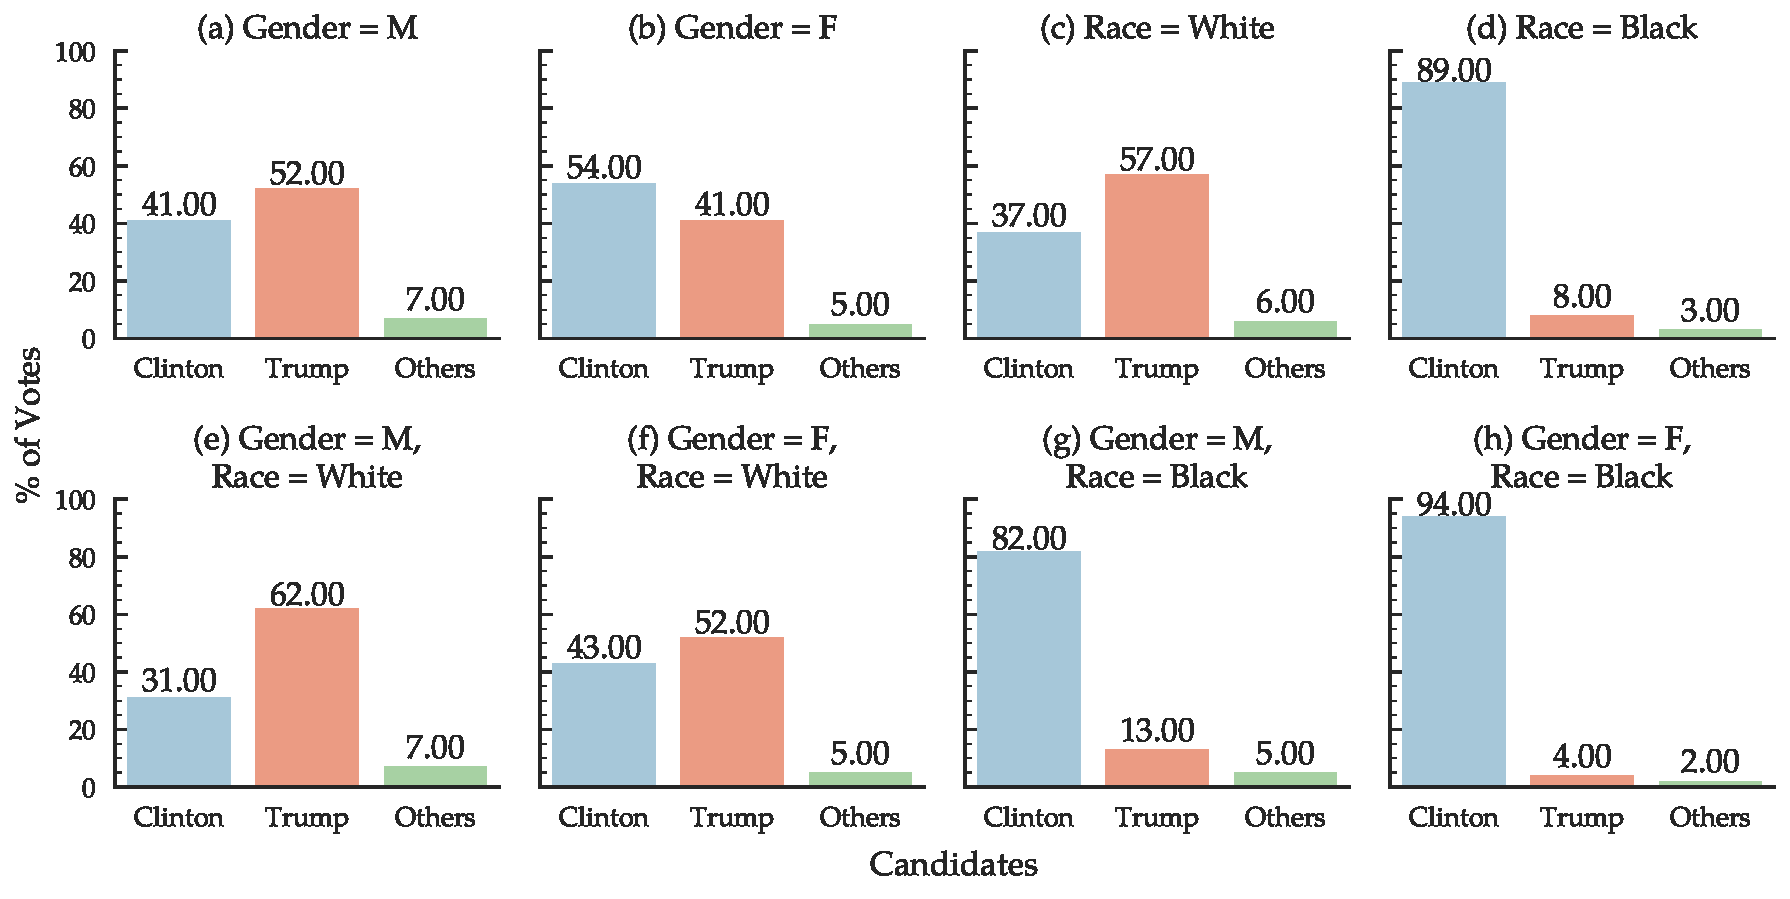
\includegraphics[scale=0.55]{figures/US_Election_Example.pdf}
\caption{A set of visualizations from the 2016 Election polls. These visualizations show the percentage of votes for three candidates (Donald Trump, Hilary Clinton, and Others) in different demographic groups (based on race and gender).}
\end{figure*}

\section{Introduction}

%\hdev{Let's take a step back, and look at the current flow in introduction. In the first paragraph, we vaguely motivate what can be considered as collective insights. In second paragraph, we try to connect the idea of collective insights with the challenges of data subset exploration. In third paragraph, we introduce two concepts: visual summarization, and distribution awareness. We do not clearly state what these two means. There's an example that conveys what could be captured through pattern or trend mining. In the fourth paragraph, we present an example to convey some specific challenges of visual summarization. The fifth paragraph states our contributions. My suggestion is to immediately jump into business by saying what we mean by distribution awareness, why is it important, and why is this challenging. We have the contents lying around already, it's just a matter of clearly stating these three aspects, preferably without using new abstractions.}

Common analytics tasks, such as causal inference, feature selection, and outlier detection requires studying the distributions or patterns at different granularities of data [Refs]. For example, a campaign manager may study the voting patterns in different demographics (based on race, gender, social class etc.) using the 2016 US election exit polls\footnote{\url{https://edition.cnn.com/election/2016/results/exit-polls}} to identify the nonconformist demographic groups. Visual analysis is the \emph{de facto} approach for performing such analytics tasks [Refs], where an analyst constructs visualizations to capture the distributions at different subsets of data. The goal of this visual analysis is to extract meaningful insights---when a set of visualizations along with human interpretation leads to informative and interesting facts arising from the distributions.

However, without knowing \textit{what} subset of data contains an interesting distribution, manually exploring all possible data subsets can be tedious and inefficient for an analyst. For example, the aforementioned campaign manager could construct bar charts for different demographics, where x-axis shows the election candidates and y-axis the percentage of votes for these candidates. Subsequently, he could compare these bar charts to understand how voting pattern changes across different demographics. Both of these exercises, first, constructing the large number of visualizations corresponding to all possible data subsets, and then, navigating through this large space of visualizations to draw meaningful insights is challenging. Currently, there is no systematic way to perform these exercises. 

To this end, we present \system, an interactive visualization summarization system that automatically selects a small set of visualizations to summarize the data distributions within a dataset in an informative manner. When analysts inspect informative visualizations that cover these insights, they associate particular sets of attributes to typical trends and observed patterns. We define this aspect of dataset understanding as \emph{distribution awareness}. For example, we observe that in Figure~\ref{fig:elections_example}, most of the visualizations has `Clinton' and `Trump' as comparably-sized bars with `Others' being a small fraction of the overall (a,b,c,e,f), whereas visualizations involving the Black population is highly skewed towards `Clinton' (d,g,h). Since human analysts have limited memory and attention, it is often impossible to visualize all possible data subsets. An ideal summarization system should display visualizations that enables users to gain maximal distribution awareness of the typical trends within a dataset. 

%Even after constructing the visualizations for all possible data subsets, which itself is a daunting task, currently there is no systematic way for our campaign manager to make sense of or even navigate through this large space of possible visualizations to draw meaningful insights. 

%\par The goal of visual analysis is to extract meaningful stories or insights from the data. Individual visualizations represent simple ``factoids'' portraying one aspect of the data. Meaningful insights arise when a group of factoids work in conjunction, along with human interpretation, to produce informative and interesting facts. 
%\par However, without knowing \textit{what} subset of the data would be interesting to visualize, manual drill-downs and roll-ups on all possible filter combinations can be tedious and inefficient for analysts. In many data analytics scenarios, analysts have an x and y axis of interest and want to explore data subsets corresponding to different filtering criteria. For example, a campaign manager may be interested in looking at bar chart visualizations of x as the voted candidate and y as the percentage of votes for the 2016 US elections exit polls with different filter combinations on demographics information, such as gender, income, race, states, and responses to different survey questions\footnote{\url{https://edition.cnn.com/election/2016/results/exit-polls}}. The analyst would have to compare across a combinatorially large space of different data subsets by iteratively changing the filter criterion of a visualization to understand how the relationship between the x and y variables change across data subsets. Even if the analyst had plotted visualizations for all possible data subsets, currently there is no systematic and effective way for an analyst to make sense of and navigate through the large space of possible visualizations to draw meaningful insights. 
%\par To this end, we present \system, an interactive visualization summarization system that automatically selects a small set of visualizations to summarize the data distributions within a dataset in an informative manner. When analysts inspect informative visualizations that cover these insights, they associate particular sets of attributes to typical trends and observed patterns. We define this aspect of dataset understanding as \emph{distribution awareness}. For example, we observe that in Figure~\ref{fig:elections_example}, most of the visualizations has `Clinton' and `Trump' as comparably-sized bars with `Others' being a small fraction of the overall (a,b,c,e,f), whereas visualizations involving the Black population is highly skewed towards `Clinton' (d,g,h). Since human analysts have limited memory and attention, it is often impossible to visualize all possible data subsets. An ideal summarization system should display visualizations that enables users to gain maximal distribution awareness of the typical trends within a dataset. 
%\par However, finding effective visualizations to summarize a dataset is not as trivial as picking individual visualizations that maximizes some statistical measure, such as deviation~\cite{Vartak2015}, coverage~\cite{Sarvghad2017}, or significance testing~\cite{Anand2015}, which can often result in misleading summarizations. Consider an elections campaign manager who is allocating the advertisement budget to be spent on different demographic populations to target for an upcoming election by investigating the voting patterns across different demographic groups. He performs a randomized permutation testing between the gender and race attributes and finds that the voting pattern of black females is drastically different from the voting pattern of general female population and allocates the his advertisement funds to target the black female population. \dor{Himel, can you check if this example makes sense? or should we say chi2? chi2 just give you columnar correlation info not at the attribute-level info? although probably only a deviation based comparison can give you a comparison like this.} While black females do defy the trends of general females, the comparison is incomplete, since it ignores the fact that black females follows very closely to the distribution of the voting behavior of the black population, so the proper subpopulation to target should be the black population rather than the more specific black female population.
%\par The above example showcases a scenario where the selection of an improper reference (female) for comparing the visualization (black female) against results in misleading insights. In \system, we formulate an objective where a visualization is \emph{actually} interesting when it deviates from and can not be explained by \emph{even} its most informative reference. \dor{can we add an example here?} Our user study results described in Section~\ref{sec:userstudy} shows that this notion of informative interestingness can guide an analyst towards more meaningful stories for further investigation. 
\par The contribution of this paper include: 
\begin{denselist}
\item Proposing the novel problem of visualization summarization and use cases highlighting the importance of \textit{distribution awareness} in dataset understanding (Section~\ref{sec:distributionaware}), %inform  visualization understanding and analytical tool designs
\item Formulating the structure and utility of the visualization search space (\emph{lattice}) using a user expectation model motivated by our formative study (Section~\ref{sec:datamodel}),
\item Designing efficient algorithms and optimizations to identify a set of informatively connected interesting visualizations (Section~\ref{sec:system}),  
\item Presenting an interactive visualization dashboard interface that adopts a simple and intuitive hierarchical lattice layout (Section~\ref{sec:interaction}),
\item Demonstrate the efficacy of our system through a user study evaluation (Section~\ref{sec:userstudy}).
\end{denselist}
\section{Related Works}
\subsection{Data Exploration of OLAP Data Cubes}
\cite{Sarawagi1998} introduced the problem that manual, unguided search for seeking interesting patterns in a datacube is inefficient and requires large numbers of OLAP operations. They propose a discovery-driven approach to data exploration to simplify the search for \textit{exceptions} in the data, based on precomputed statistics regarding how surprising a data cube cell is, relative to neighboring cells at the same level of aggregation, at levels of aggregation below the cell, and along the drill-down path.  \cite{Sarawagi1999} presents an OLAP operator that summarizes the reasons for variation in a data view, by computing the information theoretic distance between the immediate parent and its child nodes.
\par While \cite{Sarawagi1998} takes a more data-driven approach of finding exceptions intrinsic to a given datacube,  \cite{Sarawagi2000} envisions a more user-centric application where the comparisons are based only on parents of seen visualization. The user's expectation regarding an unseen visualization is based on the maximum entropy principle where the relationships between the attributes should be maximally uniform across all dimensions, while being consistent with constraints from seen visualizations. The visualization that deviates the most from the user expectation is regarded as an ``interesting" visualization. They take an iterative approach to find the unique solution for the expected values for each attribute from the constrained maximum entropy problem and employ several optimization strategies (reusing computed values, sharing storage of contiguous regions, pruning constraints that subsumes one another or with little influence). Our coverage-based models improve on the iterative approach in providing a tighter constraint to the variable regions of the bars.
\subsection{Visualization recommendation}
\par Despite the large body of work that recommends informative visualizations given pre-selected data attributes and aggregations, the data selection problem is a more important problem in exploratory data analysis, since the analysts have to figure out which groups of data attributes would be of interest in order avoid manual exploration of the data.  \cite{Anand2015} used randomized permutation tests to automatically select categorical variables to partition upon to determine which displaying multiple views of a multidimensional dataset. \cite{Vartak2015} developed a system that finds interesting visualizations by a distance-based measure between the user's query view and reference view,  given a query of interest.\cite{Wongsuphasawat2016} presents a mixed-initiative system where the users direct the variables of interest and the system suggests other variables that may be potentially interesting to the user. Since this is a mixed-initiative system rather than the automatic recommendation engine we envision in our work, the system only ``looks ahead"  by only one variable at a time. Their goal is to promote breadth-oriented data exploration rather than helping users find interesting visualizations.
\subsection{Storytelling with visualization sequences}
- the issue of surprisingness metric and ---- have been examined before for viz, but none have looked at data subset lattice specifically for viz

While most papers on visualization sequences and storytelling have focussed on using a linear layout to present the visualizations (motivated by slidedecks), ours is the first to present visualization in a graph-layout shown to be more interpretable for drill-down, roll-up type operations.
%!TEX root = main.tex
\section{Data and User Models\label{sec:datamodel}}

In this section, we first describe our data model by reporting our data, visualization and query setup, and the underlying lattice of data subsets. We then discuss how analysts explore the lattice through a formative user study, and introduce our user model based on the findings of this study. Finally, we present our problem of finding an informative-and-interesting set of visualizations from the lattice.

\subsection{Structure of visualization stories\label{sec:structure}}
%While the user model used in \system aligns with these findings, our work is the first to present a system that recommends a connected visualization sequence in a hierarchical layout summarizing the space of data subsets.

% \subsection{Data Model}
% We start by discussing the data, visualization and query setup.

% \textbf{Data.}
%\npar \stitle{Data:} We assume that we are operating on a dataset consisting of a single relational table $R$ with dimensions and measure attributes. Our approach also generalizes to multiple tables obeying a star or a snowflake schema \cite{levene2003snowflake}, but we focus on the single table case for ease of presentation.

%\textbf{Visualization.} We define the notion of a visualization for our problem. There are different visualization types such as bar charts, scatter plots, and trend lines, but across all types, a visualization can be defined using five main components: (i) the x-axis attribute(s), (ii) the y-axis attribute, (iii) the subset of data used, (iv) the binning and aggregation functions for the x- and y- axes, and (v) the type of visualization (e.g., bar chart, scatter plot).

%\textbf{Visualization.} We define the notion of a visualization for our problem. In our setup, a visualization can be defined using five main components: (i) the x-axis attributes, (ii) the y-axis attribute, (iii) the subset of data used, (iv) the aggregation function for the y- axis, and (v) visualization type, e.g., bar chart. For example, the Election Polls dataset (used for Figure 1) has four attributes: {\tt Id} (random id for each voter), {\tt Gender} (of the voter), {\tt Race} (of the voter), and {\tt Candidate} (who the voter elected); and the first visualization in Figure 1 can be defined using these attributes as: (i) {\tt Candidate}, (ii) {\tt Id}, (iii) {\tt Gender = Male}, (iv) {\tt Percentage}, (v) {\tt Bar}. We can similarly define other visualizations from this dataset. Note that, even for the same x- and y- axis attribute, aggregation function (for y- axis), and chart type (say Bar), we have a different visualization for each data subset. In Figure 1, we present all except one (the overall) bar charts that show the distribution of vote (corresponding to {\tt Percentage} of {\tt Id}) for 2016 US election candidates (values of {\tt Candidate}), for different demographic groups (the combination of {\tt Gender} and {\tt Race}).
\npar \stitle{Data Model:} We consider the common visual analytics scenario where a dataset consists of a relational table $R$ with \textit{dimensions} attributes to be filtered upon and \textit{measure} attributes to be aggregated upon. A visualization of this dataset consist of: (i) {\tt X}: x-axis attributes, (ii) {\tt Y}: y-axis attribute, (iii) {\tt C(Z)}: filter constraints that specify the data subset, (iv) {\tt A}: aggregation functions for the x- and y- axes. For example, the aforementioned elections dataset has four attributes: voter's {\tt ID}, voter's {\tt Gender}, voter's {\tt Race}, and the {\tt Candidate} that the voter elected for. As shown in Figure \ref{fig:elections_example}, even for the same x- and y- axis attribute, aggregation, and chart type, there can be different visualizations corresponding to different demographic groups (the combination of {\tt Gender} and {\tt Race}). Such visualizations can be written as \textsc{SQL} query: {\tt SELECT X, A(Y) FROM R WHERE C(Z) GROUP BY X}.\footnote{Note that our method directly applies to all counting-based aggregation functions on {\tt Y}, such as \textsc{COUNT}, \textsc{SUM}, \textsc{AVERAGE}, \textsc{PERCENTAGE}. However, our method is not directly applicable to other aggregate functions, such as \textsc{MIN}, \textsc{MAX}, \textsc{MEDIAN}.}
% \dor{possibly ignore discussion of visualization type and just say we focus on bar chart since its most common and cite.} , and (v) visualization type (e.g., bar chart, scatter plot)
\npar Given a set of visualizations $V$ with the same $X$ and $Y$ and different $C(Z)$, we extend the set-theory based \emph{containment} relationships for data subsets and organize the visualizations into a \textit{lattice} as depicted in OLAP data cube literature~\cite{Xin2007}. A visualization $V_i$ (defined by filters $C_a$) is a \textit{parent} of the visualization $V_i^j$ (defined by filters $C_b$) if $C_b$ can be obtained from $C_a$ by adding one additional filter constraint. For example in Figure~\ref{fig:elections_example}, the visualizations (b) Female and (d) Black are the parents of the (h) Black Female visualization. Based on the containment relationship of visualizations, we can organize the visualizations from $V$ to form a lattice, as exemplified in Figure~\ref{fig:lattice}. The lattice contains all visualizations with same x- and y- axes for different data subsets, arranged based on the parent-child relationships between visualizations. The choice of a filter-based data lattice is supported by research in visualization storytelling showing that people prefer visualization sequences structured hierarchically with increasing levels of aggregation~\cite{Kim2017,Hullman2017,Hullman2013}. Given this structure describing the space of possible visualizations, we will now discuss how the edge utility of visualizations in this lattice is defined.
% \textbf{Containment.} Given a data subset defined by a set of constraints $C = \{Z_1 = z_1, \ldots, Z_n = z_n\}$, expanding $C$ by adding one or more new constraints will generate a new data subset that is contained within the former subset. An ancestor-descendant relationship exists between these data subsets. Specifically, a data subset defined by constraints $C_a$ is an ancestor of a data subset defined by constraints $C_b$, if and only if $C_b \subsetneqq C_a$. Further, a data subset defined by constraints $C_a$ is a parent of a data subset defined by constraints $C_b$, if and only if $C_b \subsetneqq C_a \land \mid C_a \mid - \mid C_b \mid = 1$. For example, given a dataset with three attributes {\tt \{P, Q, R\}}, the data subset defined by constraints {\tt \{P = 0,Q = 1\}} has two parents--- the data subset defined by constraint {\tt \{P = 0\}} and the data subset defined by constraint {\tt \{Q = 1\}}.
% \textbf{Lattice.} Based on the containment relationship, we can organize the data subsets of a given dataset to form a hierarchy. This hierarchy of data subsets is overlaid on top of the lattice of attribute combinations. For the rest of the paper, we refer to this data subset hierarchy (overlaid on top of attribute lattice) as \emph{lattice}. In Figure~\ref{fig:lattice} we show the lattice of data subsets for a dataset with three attributes {\tt \{P, Q, R\}}, where we highlight the data subsets that belong to the same attribute combination with the same color. For example, all data subsets with three filters (at the lowest level of hierarchy) belong to the same attribute combination {\tt \{P, Q, R\}}, and are highlighted in gray.

\begin{figure*}[ht!]
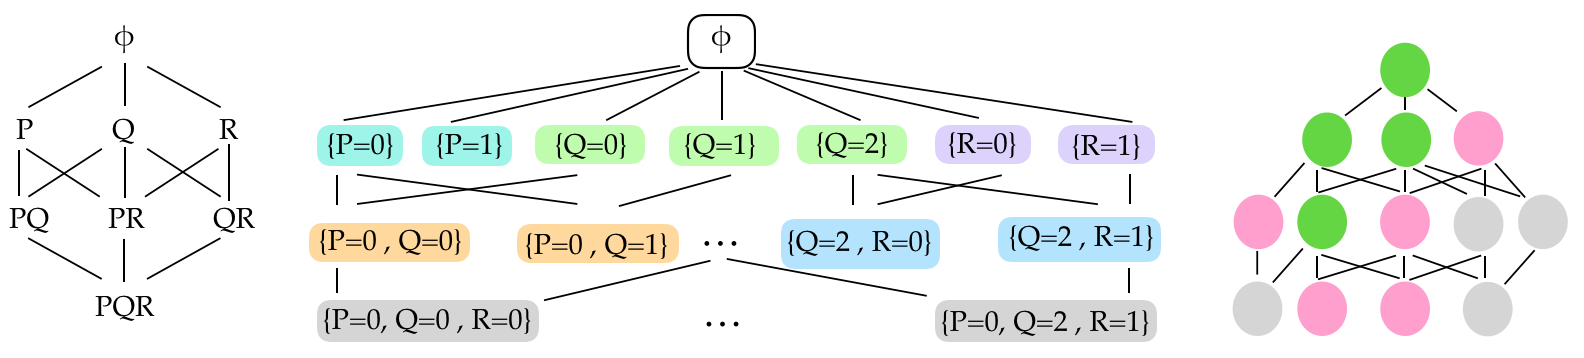
\includegraphics[width=\linewidth]{figures/lattice_frontier.png}
\caption{Left, Middle: Example data subset lattice for a dataset with three binary attributes {\tt \{P, Q, R\}}. The data subsets that belong to the same attribute combinations are highlighted with same color. $\phi$ represents the overall distribution (where no filter conditions is applied). Right: Toy example demonstrating the notion of ``frontier''. Green nodes are selected in the dashboard. The neighbors of the set of selected green nodes are the frontier nodes, shown in pink. Other unpicked nodes in the lattice are shown in gray.}
\label{fig:lattice}
\end{figure*}
We now extend the concept of \emph{containment} for visualizations defined according to our setup.

% \textbf{Viz Containment.} Let $V$ be the set of visualizations (of same type) that show the same $X$ and $Y$ for different $C(Z)$. Given a visualization $V_i \in V$, a parent of $V_i$, $V_i^j$ ($V_i^j\in V$) is a visualization that corresponds to a parent data subset of the former. In Figure~\ref{fig:elections_example} we present three visualizations that show the distribution of votes for 2016 US election candidates in three demographic groups: (i) female voters, (ii) black voters, (iii) black female voters. As per the parent-child relationship among the data subsets, the visualizations corresponding to (i) and (ii) are parents of the visualization corresponding to (iii).

% \begin{figure}[bht]
% \centering
% 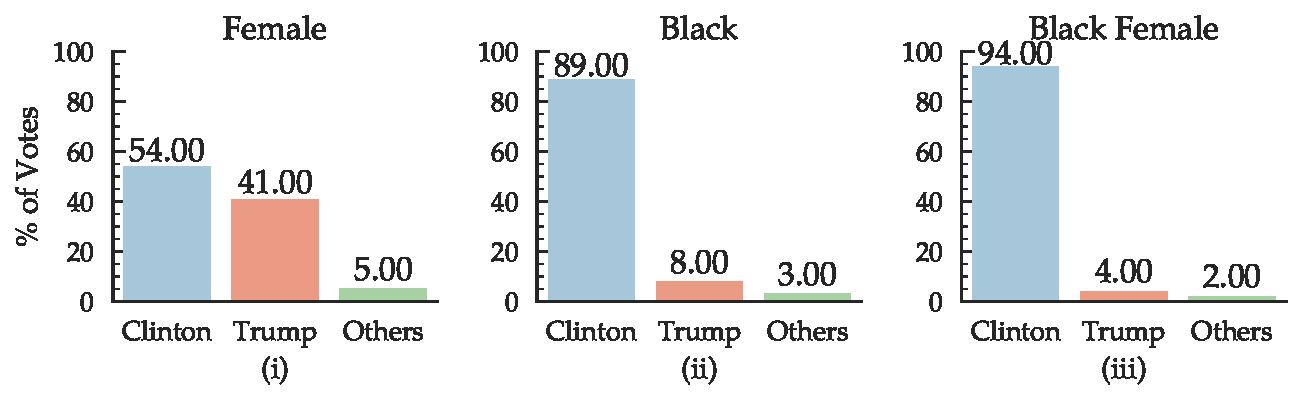
\includegraphics[scale=0.4]{figures/US_Election_Parent_Child.pdf}
% \caption{Parent-child relationship amongst visualizations that show the distribution of votes for 2016 US election candidates in three demographic groups: (i) female voters, (ii) black voters, (iii) black female voters.}
% \label{fig:elections_example}
% \end{figure}

%\haz{Perhaps it will look better if have (iii) in a new line (and centered) to quickly reflect the parent-child relationship.}\dor{Considering that this will take up more space also not sure whether not sure we should mix up the problem formulation with the model itself. Himel?}

% \textbf{Viz Lattice.} Based on the containment relationship of visualizations, we can organize the visualizations from $V$ to form a lattice. This lattice contains all visualizations (of same type, e.g., bar charts) that show the same x- and y- axes for different data subsets, and arranges them as per the parent-child relationships between data subsets. Our goal is to traverse this lattice of visualizations, and identify informative and interesting visualizations.

\subsection{Utility of Visualizations: User Expectation Model\label{sec:utility}}
In order to identify which visualizations should be picked from the lattice, we conduct a formative user study
to study how the presence of one or more of observed parent in the visualization lattice affects an analyst's perception of an unseen visualization. Using these findings, we then model the effective utility of displaying an unseen visualization to a user in the context of seen visualizations.% by defining metrics of \textit{interestingness} and \textit{informativeness}.
%to study how analysts interpret parent-child relationships in a visualizations lattice, and then model the effective utility of displaying an unseen visualization to a user in the context of seen visualizations.
%\textbf{Top Down Traversal.} We observe that, while exploring a dataset, users first look at the top level visualizations before looking at the next level \cite{Kim2017, Hullman2013}. Further, the data distributions learnt from the top level visualizations induce user expectation for the next level. For example, in Example 1, a journalist is likely to examine the voting trends of female or black voters before examining the voting trends of black female voters, and his/her expectation of black female voters would be affected by the observed reference(s) (female or black voters). Based on these two observations, we model user expectation $\hat{V_i}$ corresponding to an unseen visualization $V_i$ based on its seen/observed parents $O(V_i) = \{V_i^1, \ldots, V_i^\lambda\}$ in the visualization lattice.

\stitle{Formative User Study:} %We conducted a user study to understand how a user's perception of an unseen visualization is affected by one or more of its observed parents.
We recruited 9 participants in a study to predict the distribution of an unseen visualization with two constraints. Participants were asked to make a prediction regarding an unseen visualization after seeing the first parent displayed and subsequently after seeing the second parent displayed. For the chosen visualization parents, the first parent have data distributions that very closely follows that of the unseen visualization, whereas the second parent differs greatly from the unseen visualization. In this between-group study, one group of participants (G1) were shown the first parent followed by the second parent, whereas another group of participants (G2) were shown the second parent followed by the first parent. We examined how users form their expectation in presence of these observed parents. The results are summarized in Figure \ref{fig:formative_study}. Our main findings are: (1) participants naturally form their expectations based on one or more observed parents; (2) seeing a parent that well describes the unseen visualization leads participants to better estimate the unseen visualization; (3) in absence of an informative parent, participants can be misled to form an inaccurate expectation; (4) in presence of multiple parents, the variance of expectation increases.
\begin{figure}[h!]
\centering
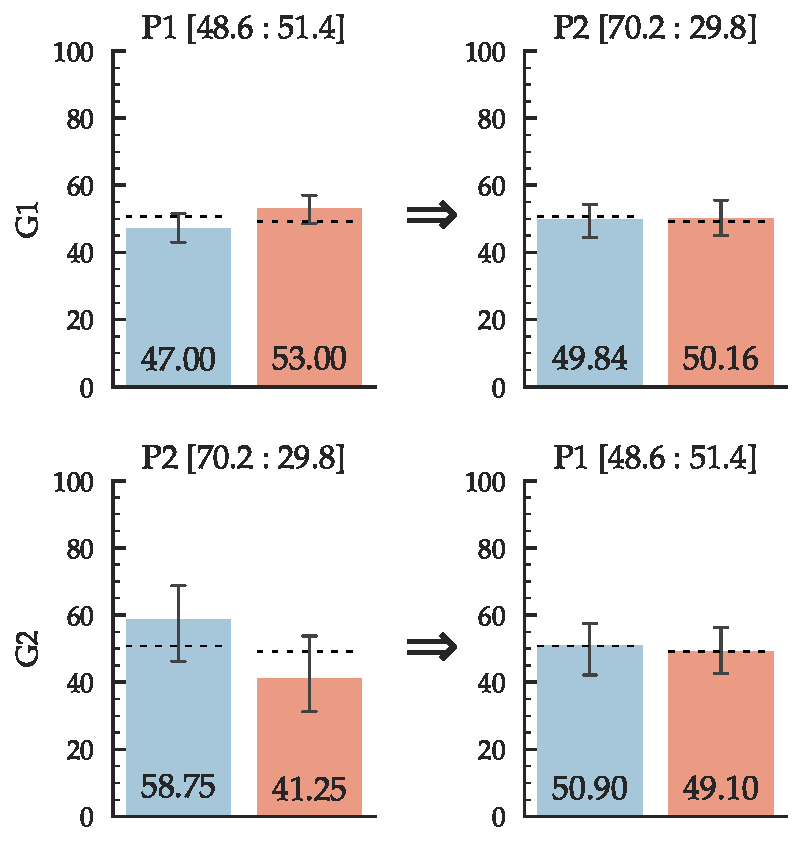
\includegraphics[width=\linewidth]{figures/Formative_Study.pdf}
\caption{Bar charts and error bars showing the mean and variance of participants' estimated distribution during the formative user study. Group 1 (G1) participants were shown the informative parent first, followed by the uninformative parent; whereas Group 2 (G2) participants were shown the uninformative parent first, followed by the informative parent. G1 participants closely approximated the unseen visualization immediately after seeing the informative parent. The ground truth visualization values are shown as dotted lines and printed in square brackets in the visualization title.}
\label{fig:formative_study}
\end{figure}
\npar Based on these findings, we model two aspects of the unseen-visualization and observed-parent relationship through its \textit{interestingness} and \textit{informativeness} criteria.
\stitle{Informativeness:} To model the informativeness of an observed parent in the context of an unseen visualization, we characterize the capability of the parent in predicting the unseen visualization. As highlighted in finding (2), an observed parent is \emph{informative} if its data distribution closely follows the data distribution of the unseen child visualization, since the visualization helps the analyst form an accurate mental picture of what to expect from the unseen visualization. Specifically, we formulate the informativeness of an observed parent $V_i^j$ of an unseen visualization $V_i$ as the similarity between their data distributions measured using a distance function $D(V_i, V_i^j)$. The most informative parents $V_i^*$ of an unseen visualization $V_i$ are the ones whose data distributions are most similar to the unseen.
\begin{equation}
    V_i^*=\underset{V_i^j}{argmin}\ D(V_i, V_i^j)
\end{equation}
Since our finding (4) demonstrates how seeing multiple parents can lead to worser visualization understanding, we allow users to specify a threshold $\theta$ to control the degree of similarity for which a parent can be declared as an informative, such that the distance $D(V_i, V_i^{*, \theta})$ corresponding to the informative parents $V_i^{*, \theta}$ are at least $\theta\%$ close to its most informative parent:
\begin{equation}
    V_i^{*, \theta} = \{V_i^j : \frac{D(V_i, V_i^*)}{D(V_i, V_i^j)} \leq \theta\}
\end{equation}
%Since declaring a parent as informative can vary depending on its similarity with the unseen compared to other parents, we allow the user to specify a threshold $\theta$, which we expect to be close to 1.0, such that the similarity score $S(V_i, V_i^{*, \theta})$ corresponding to the informative parents $V_i^{*, \theta}$ are at least $\theta\%$ of that of the most informative parents'.
For example, if $\theta = 0.8$, all parents of $V_i$ whose similarity scores are at least 80\% of that compared to $V_i^*$ are deemed as \textit{informative}. In Figure~\ref{fig:elections_example}, while both visualization (b) and (d) are considered parents of visualization (h), only visualization (d) (Black) are considered the informative parent of visualization (h) (black female population), for any values of $\theta \geq 11\%$ via the Euclidean distance metric. %the visualization corresponding to black voters is the most informative parent of the visualization corresponding to black female voters. For $\theta <= 0.11$, the former remains the only informative parent of the latter.

\stitle{Interestingness:} While informative parents contribute to the prediction of an unseen visualization, the most interesting visualizations to recommend are those for which \emph{even the informative parents fail to accurately predict the visualization}. \dor{Can we justify this based on our findings?} To model the interestingness of an unseen visualization $V_i$ in the context of an observed parent $V_i^j$, we characterize the deviation between their data distributions using a distance function $D(V_i, V_i^j)$. The unseen visualizations whose data distributions deviate from the observed informative parents are \emph{interesting}. \cut{The most interesting unseen visualizations $V_\#$ are the ones that deviate most from their observed informative parents.
\begin{equation}
    V_\#=\underset{V_i}{argmax} \ D(V_i, V_i^{*, \theta})
\end{equation}
In Figure \ref{fig:elections_example}, the most interesting visualization to recommend is the one corresponding to white female voters. This visualization significantly differs from its informative parent---the visualization corresponding to female voters.} \dor{The argmax notation not necessary since we're just using this in our utility function. The election example is not convincing, the informative parent of white female is actually white and not female. Also the differences are not too significant.}

%\noindent Additional model extensions can be added to this objective function based user specification. For example, there may be $k$ visualizations that approximately yield equal contribution to the user's expectation. For simplicity of notation, we have assumed $k=1$ in the aforementioned model. In order, a user may want to prevent the recommendation of spuriously interesting subsets of the data. We can discard visualizations that falls below a certain subpopulation size threshold.
\stitle{Subpopulation size consideration:} The danger of spurious patterns and correlations in visualizations that contain small subpopulation size is a well-known problem in exploratory analysis~\cite{Binnig2017}. We take two preventive measures to avoid including such misleading visualization in our dashboards. First, in the lattice generation process discussed in Section~\ref{sec:algorithms}, we allow users to select an `iceberg condition' \footnote{The terminology is used in the discussion of iceberg cubes in OLAP literature~\cite{Xin2007}.} ($\delta$) to adjust the extent of pruning on visualizations whose sizes fall below a certain percentage of the overall population size. Second, we downweigh the interestingness edge utility $U(V_i, V_i^j)$ between a parent $V_i^j$ and a child visualization $V_i$ by the ratio of their sizes:
\begin{equation}
    U(V_i, V_i^j) = \frac{|V_i|}{|V_i^{j}|} \cdot D(V_i, V_i^j)
    \label{edge_utility}
\end{equation}
\subsection{Problem Formulation}
Given the lattice data model and the user model for visualization utility described above, the goal of our system is to generate a dashboard by selecting $k$ visualizations from the lattice. We enforce that the generated dashboard satisfies several requirements:
 \begin{enumerate}
 	\item Dashboard must include the overall visualization (topmost visualization with no filter applied) to serve as reference to the rest of the visualizations in the dashboard.
 	\item For each visualization except for the overall, at least one of its informative parents is included within the $k$ visualizations. This excludes the uninformative parents as exemplified in black female example in the dashboard, especially since our findings 3 and 4 shows that showing multiple, improper parents can mislead the participants, resulting in a higher variance across their estimations. %enforces that every visualization shown in

  the dashboard has an informative reference to compare against to create a connected story.
 	\item The selected $k$ visualizations are collectively most ``interesting'' in presence of their informative parents as measured by the utility in Equation \ref{edge_utility}.
\end{enumerate}
 The problem of finding a connected subgraph in the lattice that has the maximum combined edge utility is  known as the maximum-weight connected subgraph problem~\cite{ErnstAlthaus2009} and is known to be NP-Complete, via a reduction from the \textsc{Clique Problem}~\cite{Parameswaran2010}. In Section~\ref{sec:algorithms}, we discuss heuristic algorithms used for deriving a locally optimal solution for ensuring interactive runtime.

%!TEX root = main.tex
\section{System\label{sec:system}}
\subsection{System Architecture}
We have implemented \system\ as a Flask web application on top of a PostgreSQL database. In Figure~\ref{system_architecture}, we present the system architecture of \system, which consists of three core modules: the traversal module, the query module, and the statistics module. The interaction manager deals with the supported user interaction described in Section~\ref{sec:interaction} and sends a request to the lattice module which  contains several algorithms for generating and traversing the visualization lattice described in Section~\ref{sec:algorithms}. For generating the visualization lattice, the lattice module passes a list of data subsets corresponding to visualizations to be generated to the query module. The query module translates these visualizations into queries, and then optimizes (by grouping) and executes the queries. The statistics module is an optional module that allows the lattice module to prune low-utility visualizations without actually generating them. Specifically, it generates coarse statistics for the unexplored visualizations based on the current list of explored visualizations. Finally, the dashboard renderer takes the resulting visualizations to be included in the dashboard and perform any rendering preprocessing procedures for display and navigation of the dashboard as described in Section \ref{sec:navigation}.
\begin{figure}[ht!]
\centering
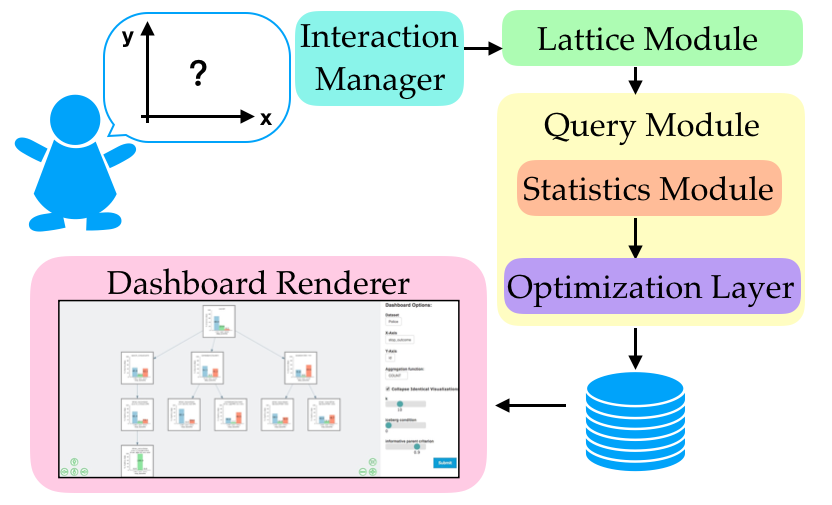
\includegraphics[width=\linewidth]{figures/system_architecture.png}
\caption{System Architecture of \system. User starts with x and y axes of interest and requests for $k$ visualizations in the dashboard. The request is processed by generating the lattice with the help of the querying module, visualization selection through the lattice traversal algorithms, and finally the dashboard is displayed at the frontend through the dashboard renderer. }%  The interaction manager translates the request to the traversal module that ???? [should we look at the offline case??]}
\label{system_architecture}
\end{figure}

\subsection{Algorithms\label{sec:algorithms}}
We give an overview of our algorithms by first discussing the approaches to generate the visualization lattice, and then presenting a high-level overview of our traversal algorithms.

\stitle{Lattice Generation.} Our system supports two variants of traversal algorithms based on the lattice generation procedure---offline variants that first generate the complete lattice and then work towards identifying the maximum utility solution, and online variants that incrementally generate the lattice and simultaneously identify the solution. The offline variants are appropriate for datasets with a small number of low-cardinality attributes, where we can generate the entire lattice in a reasonable time; whereas the online variants are appropriate for datasets with large number of high-cardinality attributes, where we incrementally generate a partial lattice.

%In most cases, the lattice contains a large number of visualizations due to the presence of many attributes or high-cardinality attributes in the dataset. In such cases finding an optimal solution is computationally challenging.

\stitle{Lattice Traversal.} Given the materialized lattice, the objective of the traversal algorithm is to find the connected subgraph in the lattice that has the maximum combined edge utility. Here, we discuss the \textit{frontier greedy} algorithm which is used for generating the dashboards for our user study and defer our discussion on the details of other algorithms that we have developed to the technical report.
% \begin{figure}[ht!]
% \centering
% 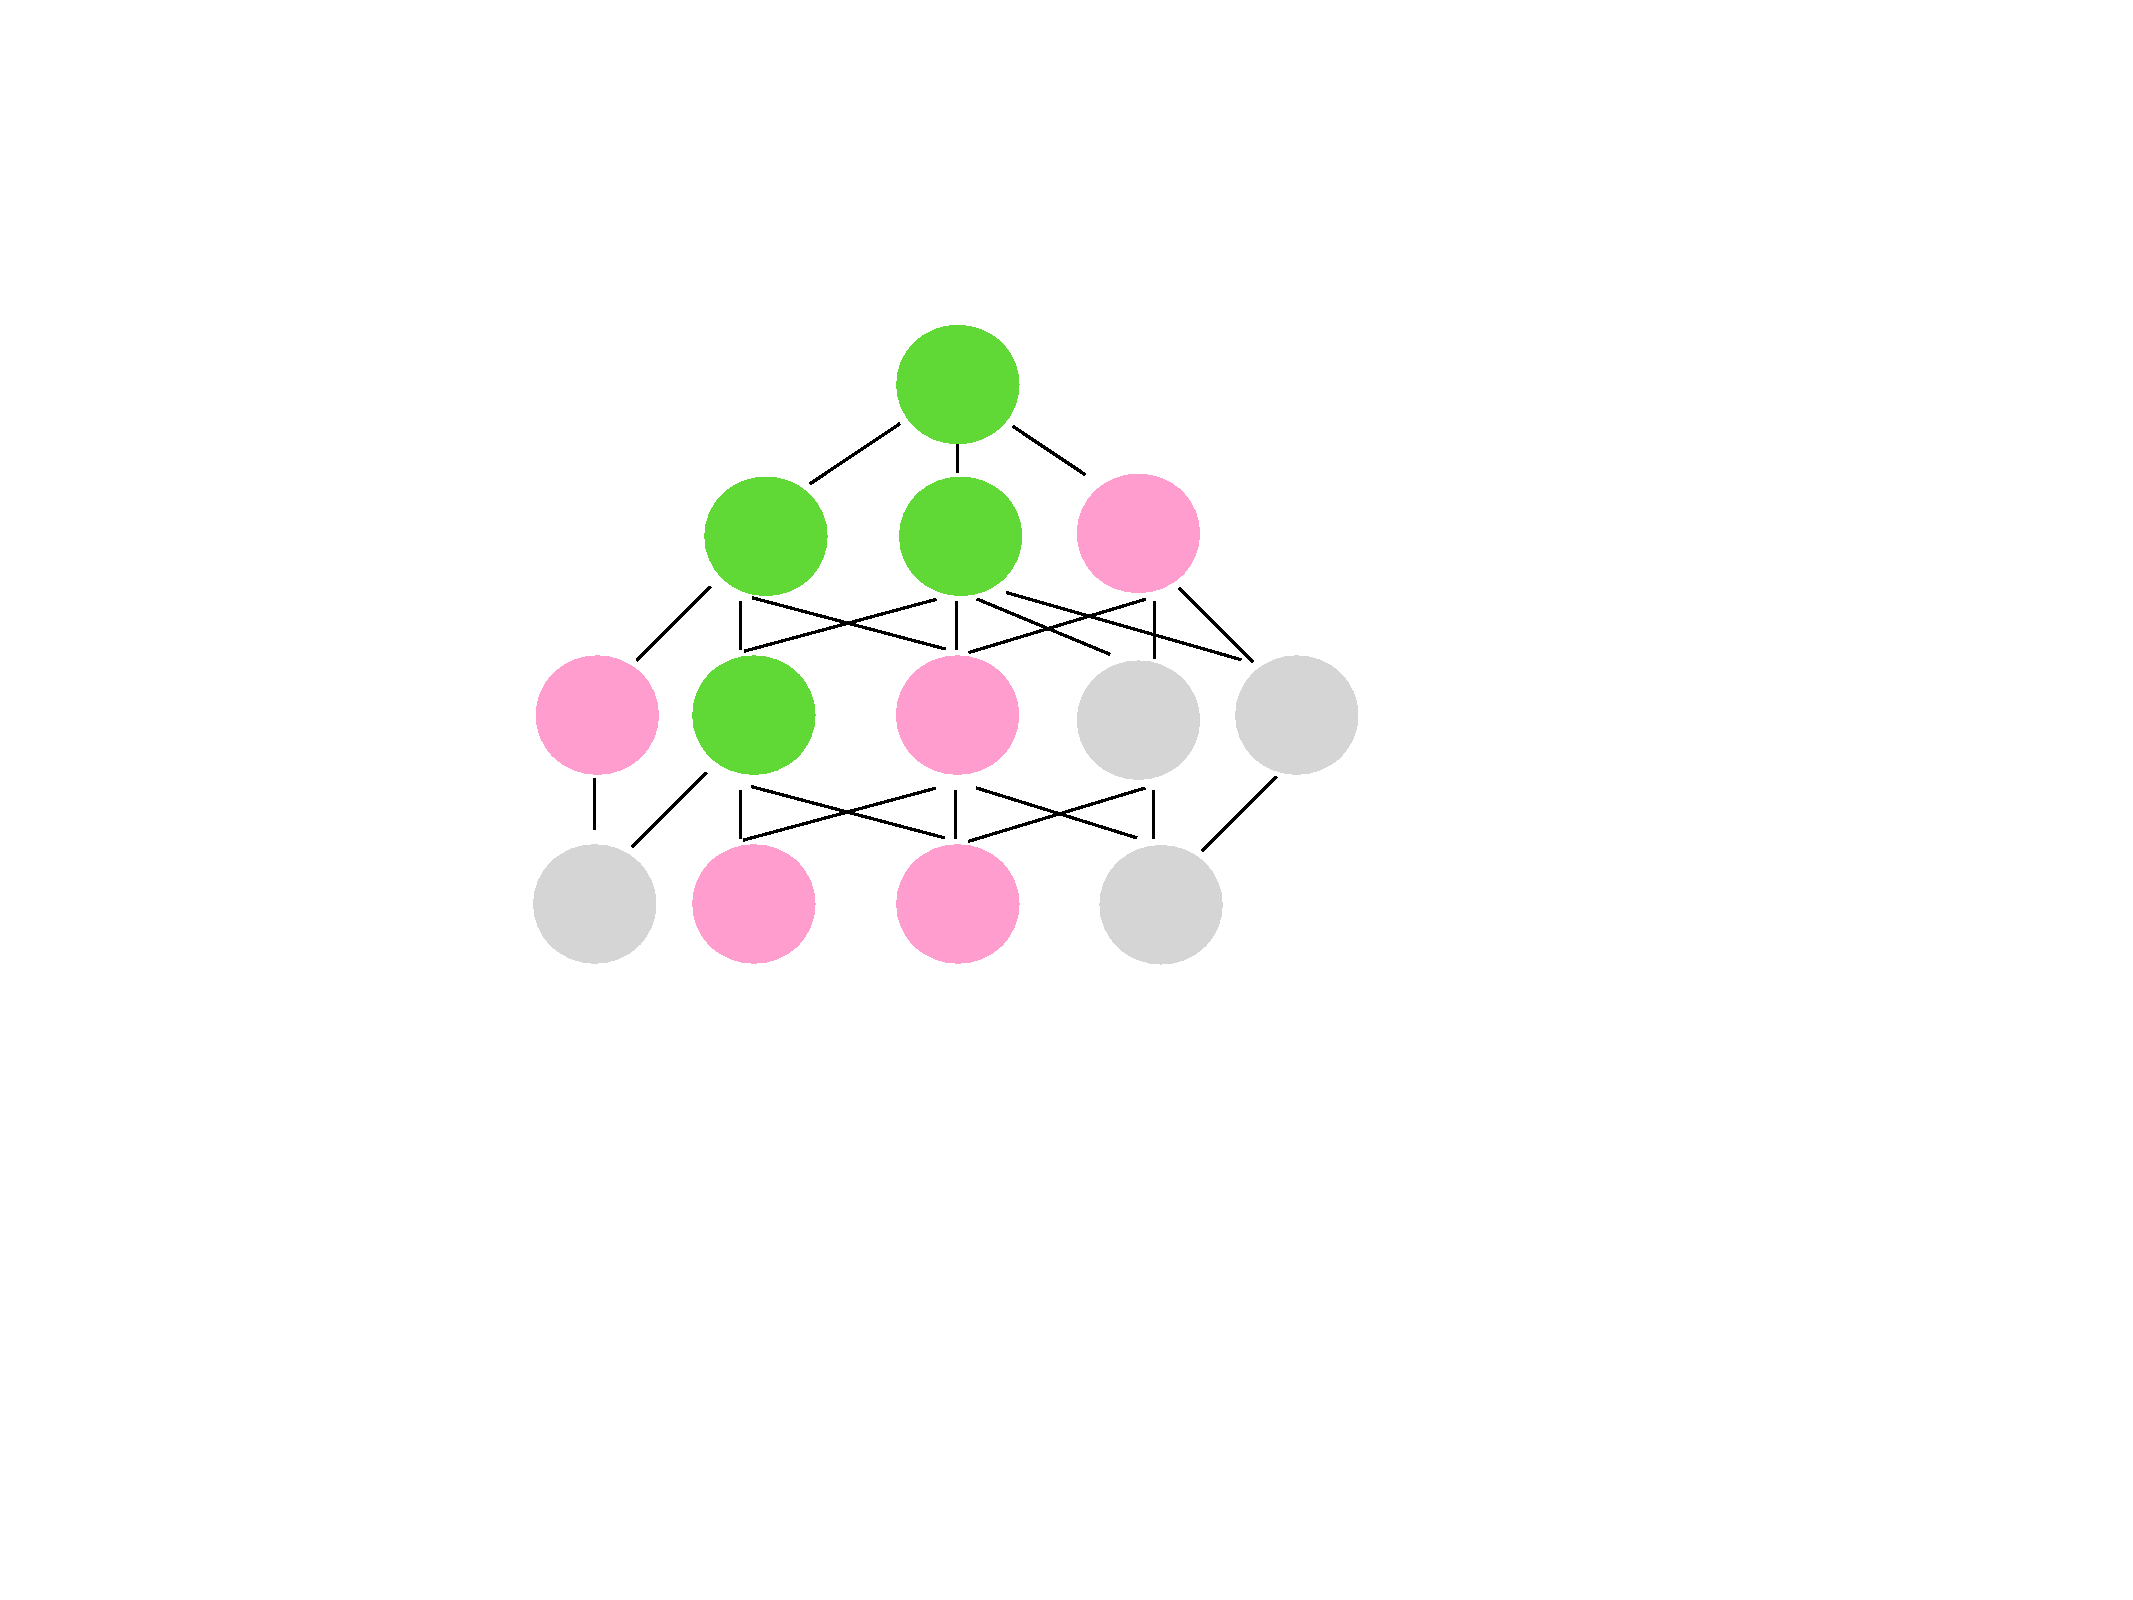
\includegraphics[width=0.4\linewidth]{figures/frontier.pdf}
% \caption{Toy example demonstrating the notion of ``frontier''. Nodes that have been picked to include in the dashboard are colored green. The neighbors of the set of picked nodes are the frontier nodes, shown in pink. Grey nodes are other unpicked nodes in the lattice.}
% \end{figure}
%We devised two classes of heuristics algorithms, namely, frontier-based algorithms, and path-merging algorithms. These algorithms are guaranteed to find a solution that satisfies the constraints of our problem, except for the optimality.
\techreport{The frontier-based algorithms traverse the lattice from root to downwards, incrementally adding new nodes (visualizations) to the current solution (dashboard) till it reaches the maximum capacity $k$. To achieve this, the algorithms maintain a list of candidate nodes---called \textit{frontier} nodes---any of which can be added to the current solution since their informative parent is already present in the solution. At each step, the algorithms add a node from frontier to the current solution, and update the frontier accordingly.  The frontier based algorithms can be further categorized into three types based on their node selection strategy (from frontier), namely greedy algorithm, random walk algorithm, and probabilistic algorithm. The greedy algorithm picks the current best node from frontier (thus concentrates on exploitation), random walk algorithm picks a random node (thus concentrates on exploration), and probabilistic algorithm picks a random high-utility node (thus trades off between exploration and exploitation).}
\par As described in Algorithm \ref{algo:frontier_greedy}, our algorithm obtains a list of candidate nodes known as the \textit{frontier} nodes (pink in Figure\ref{fig:lattice} left), which encompasses all neighbors of nodes in the existing subgraph solution. Any of the nodes in the frontier can be added to the current solution since their informative parent is guaranteed to be present in the solution. The \texttt{getFrontier} function scans and adds all children of leaf nodes of the current dashboard as part of the frontier. In the online version, it additionally checks for each child whether its informative parent is present in the current dashboard. At each step, our algorithm greedily picks the node with the maximum utility from the frontier to the current solution, and updates the frontier accordingly.

\techreport{The path merging algorithm first generate the informative paths from root to every candidate node. Then, it greedily merges the paths with high-utility to create a subgraph whose size is less than or equal to maximum capacity $k$.}

% \begin{algorithm}
%     \SetKwInOut{Input}{Input}
%     \SetKwInOut{Output}{Output}
%     \Input{Precomputed Lattice of Visualizations, $G = \{V_1, \ldots, V_n\}$}
%     \Output{A Dashboard of Size $k$, $S$}
%     $S = \{ V_{root}\}$\;
%     $F = get\_child(V_{root})$\;
%     \While{$size(S) < k$}
%     {
%     	$s_{next} = pick\_next(F)$\;
%     	$S = S \cup s_{next}$\;
%       \For{$i = 0;\ i < size(S);\ i = i + 1$}
%       {
%           $F = (F \cup get\_child(S[i])) - S$\;
%       }
%     }
%     return $S$\;
%     \caption{Frontier Based Algorithm}
% \end{algorithm}

\begin{algorithm}
  \begin{algorithmic}[1]
  \Procedure{pickVisualizations}{k,lattice}
  \State dashboard $\gets$ \{ $V_{overall}$ \}
  \While{|dashboard| < k}
      \State frontier $\gets$ getFrontier(dashboard,lattice)
      \State maxNode $\gets$ getMaxUtilityNode(frontier)
      \State dashboard $\gets$ dashboard $\cap$ \{maxNode\}
  \EndWhile
  \Return dashboard
  \EndProcedure
  \end{algorithmic}
  \caption{Frontier Greedy Algorithm}\label{algo:frontier_greedy}
\end{algorithm}

%\textbf{Greedy Algorithms:} Greedy algorithms select the locally optimal node to be added to the frontier.

%A specific implementation would need to specify a scoring function to nodes in frontier that is used to pop out the next node in each iteration. One can design a scoring function based on the trade-off between performance and complexity. In the most simple case, we can use the edge weights to score nodes in the frontier. That is, at each point we add a node with the highest interestingness value. We note that this is quite a greedy approach. Specifically, we might miss visualizations with high utility that are in deeper levels of the graph. Thus, another approach would be to extent the horizon for which we calculate a nodes utility. We denote such approach as a look-ahead approach. With a free parameter $n$, we would like to assign a score to each frontier node the corresponds to the expected utility of adding this node and $n-1$ more nodes who are its descendants. For example, we can run BFP for each node in frontier treating it as a root.

\techreport{The path merging algorithm first generate the informative paths from root to every candidate node. Then, it greedily merges the paths with high-utility to create a subgraph whose size is less than or equal to maximum capacity $k$.}

\section{User Study Evaluation}
\subsection{Procedure}
Given that our preliminary study motivated our desiderata for the metrics and constraints used in the problem formulation, we further evaluate the utility of our tool by performing a user study focusing on addressing the research questions: 
\begin{itemize}
	\item RQ1: How effective is our tool at summarizing key insights within a given dataset?
	\item RQ2: How effective is our tool in providing analysts with task-specific insights? (including understanding causal explanations, identification of interesting visualization, and finding outliers[?])
	\item RQ3: How useful are the visualizations in the recommended dashboard to analysts?
\end{itemize}
\par We recruited [NUMBER] participants who have experience working with data. This can include, but are not limited to, browsing and reading data, data cleaning and wrangling, data visualization and model building. The inclusion criteria is assessed based on a self-reporting basis in the pre-study survey. [REPORT BASIC DEMOGRAPHICS ABOUT USERS.]
\par The user study is composed of two phases. Phase one of the experiment focuses on comparing our tool against a set of baselines intended to simulate the natural sequence of visualizations that an analyst would encounter through various approaches during exploratory analysis. The baselines include: 
\begin{enumerate}
	\item Clustering (\textit{Clust}): K-Means clustering is performed on the dataset with k clusters. For each representative cluster, pick the visualization that is closest to the cluster center and display the visualization in table layout in the order of increasing number of conditions in the filter combination.
	\item Parent-Child Pairs (\textit{PC}) : Pick top k/2 parent-child pairs without enforcing informative criterion. Display as pairs of disconnected graph.
	\item Bread-First (\textit{BFS}) : k visualizations is selected in level-wise order and displayed in a graph layout. 
	\item Random (\textit{Rand}) [OPTIONAL]: k visualizations is randomly selected and display in table layout. This is intended to simulate user behavior on free-form visualization generation tool, where users add arbitrary combinations of filters to explore an unfamiliar dataset.
	%\item Direct manipulation: Allow users to add arbitrary combinations of filters and facets. Record insights until k visualizations seen. Display in table layout.
	\item Direct manipulation (\textit{DM}): Through crowdsourcing, we asked a group of expert users to add arbitrary combinations of filters and facets to create a dashboard of k visualization while given a time constraint of 30 minutes. These expert-generated dashboards are used as the DM baselines viewed by all other users in the user study. \footnote{We chose not to perform a comparison with a Tableau-like interface, since activities involved in free-form DM and our tool is fundamentally different. Direct manipulation engages users in the act of visualization construction and browsing through an iterative workflow, while our displayed dashboard only require the users to browse a set of recommendation. The confounding variable related to the cost-benefit tradeoff between visualization construction versus browsing is an unaddressed but interesting direction of research for visualization recommendation.}
\end{enumerate}
%To prevent learning effects, the ordering of the baselines will be randomized across users. 
\par At the beginning of the study, participants were provided with a dashboard from an example dataset, as well as an explanation of how the dashboard is generated. For each of the visualization dashboard generated by our tool or one of the baselines, participants are asked to mark visualizations as interesting/not interesting while explaining their reasoning for each annotation. Then, they are asked to summarize a list of insights that they have discovered after browsing through all visualizations in the dashboard. Participants also answer a set of task-specific questions related to causality and outliers[?], in the form as shown in the example [*]. These tasks are repeated for all baselines and our tool in randomized order on different datasets to prevent learning effects. At the end of phase one, participants are asked to comment on their experiences with each method, as well as the pros and cons of each of the tools. This phase of the experiment is designed to quantify the effects of RQ 1 and 2. 
\par To prevent fatigue, after a 5 minute break, the participants then proceed onto phase two of the study, where they are given [10] dashboards generated by our tool and are asked to engage in a talk-aloud exercise as they browse the recommended visualizations. This is a more open-ended study intended for addressing RQ3 that can reveal our tool show unimportant results across different datasets and/or highlight larger selection of the types of insights that can be generated from the tool. 
\subsection{Result}
%!TEX root = main.tex
\change{\section{Discussion of Study Results}}
To \bchange{further understand how participants 
made use of the recommended visualizations during their analysis}, 
we analyzed the user study \bchange{transcripts}
through an open coding process~\cite{Muller1993} by two of the authors. 
For each task in our study, we assigned a binary-valued code to indicate whether or not a participant engaged in a particular action or thought process. Table~\ref{table:thematic_summary} highlights results from thematic coding discussed in this section. We will use the notation [Participant.DatasetAlgorithm] to refer to a participant engaging with a dashboard created by an algorithm=\{1,2,3\}=\{\system, \cluster, \textsc{BFS}\} on a dataset =\{A,B\}=\{Police, Autism\}.
% \stitle{\system promotes distribution-awareness by provoking comparisons against more informative contextual references.}We first studied the thematic codes to understand how participants select contextual references for visualizations.
\subsection{The Choice of Contextual References}
\par As discussed earlier, 
analysts often make use of 
related visualizations to 
form their expectations for 
unseen \bchange{visualizations}. 
We refer to \bchange{the}
visualizations used 
for such purposes as \emph{contextual references}. 
\bchange{The appropriate choice
of a contextual reference (such as an informative parent)
is necessary to ensure the \emph{safety} of
insights derived through drill-downs.} 
To understand how ``safe'' the dashboards 
generated from each condition were, 
we examined \change{the visualizations} 
that participants compared against 
to form their expectations \change{for unseen visualizations}. 
In particular, we thematically encoded 
\bchange{the}
participants' use of contextual references 
based on \change{their} verbal explanations 
\change{for justifying} their prediction task responses. 
As shown in Table \ref{table:contextualReferenceCount}, 
in general, we find that participants make more comparisons in total using \system than compared to \cluster and \BFS.
\begin{table}[h!]
\vspace{-5pt}
\centering
	\begin{tabular}{l|rrrr|r}
	 \small{Algorithm}   &    \small{Parent} &   \small{Sibling} &   \small{Relative} & \small{Overall} &   \small{Total} \\
	\hline
	 \small{\system}     &    \cellcolor{blue!25} 12 &       8 &     0 &  11 &      \cellcolor{blue!25} 31 \\
	 \small{\cluster}     &         4 &        0 &         7 &          8 &      19 \\
	 \small{\BFS}         &         0 &        5 &         1 &          8 &      14 \\
	\end{tabular}
\caption{Out of 12 participants, the number of participants who made use of each contextual reference across the two datasets. Participant behavior shows a similar trend in individual datasets. \system participants made more comparisons in general and against parents compared to the baselines.}
\label{table:contextualReferenceCount}
\vspace{-20pt}
\end{table}
\par Participants can (and often do) make comparisons against more than one type of contextual references to obtain their prediction. We uncovered four main classes of contextual references, described below using the 
example visualization $V_i$=\texttt{\origcolor{gender=F, race=White, age=21-30}} (in the order of most to least similar to $V_i$) and illustrated in Figure~\ref{fig:reference}:
\begin{enumerate}
	\item \textbf{Parent} : Comparison against a visualization with one 
	filter removed (e.g., \texttt{\origcolor{gender=F, race=White}})
	\item \textbf{Siblings} : Comparison against a visualization that shares the same parent. In other words, the \bchange{filtered attributes are the same, but one filter has a different value}. (e.g., \texttt{\origcolor{gender=F, race=White, age=}\diffcolor{60+}})
	\item \textbf{Relatives} : Comparison against a visualization that shares some common ancestor (excluding overall), but not necessarily the same parent. \bchange{These} visualizations share at least one \bchange{common filter, but with more than one filter or filter value being different}\agp{I updated it based on what I thought this should have been--see figure for more}. (e.g., \texttt{\origcolor{gender=F, race=White, age=}\diffcolor{60+, search conducted=T}})
	\item \textbf{Overall} : Comparison against the distribution that describes the overall population (no filters applied).
\end{enumerate}
\begin{figure}[h!]
\centering
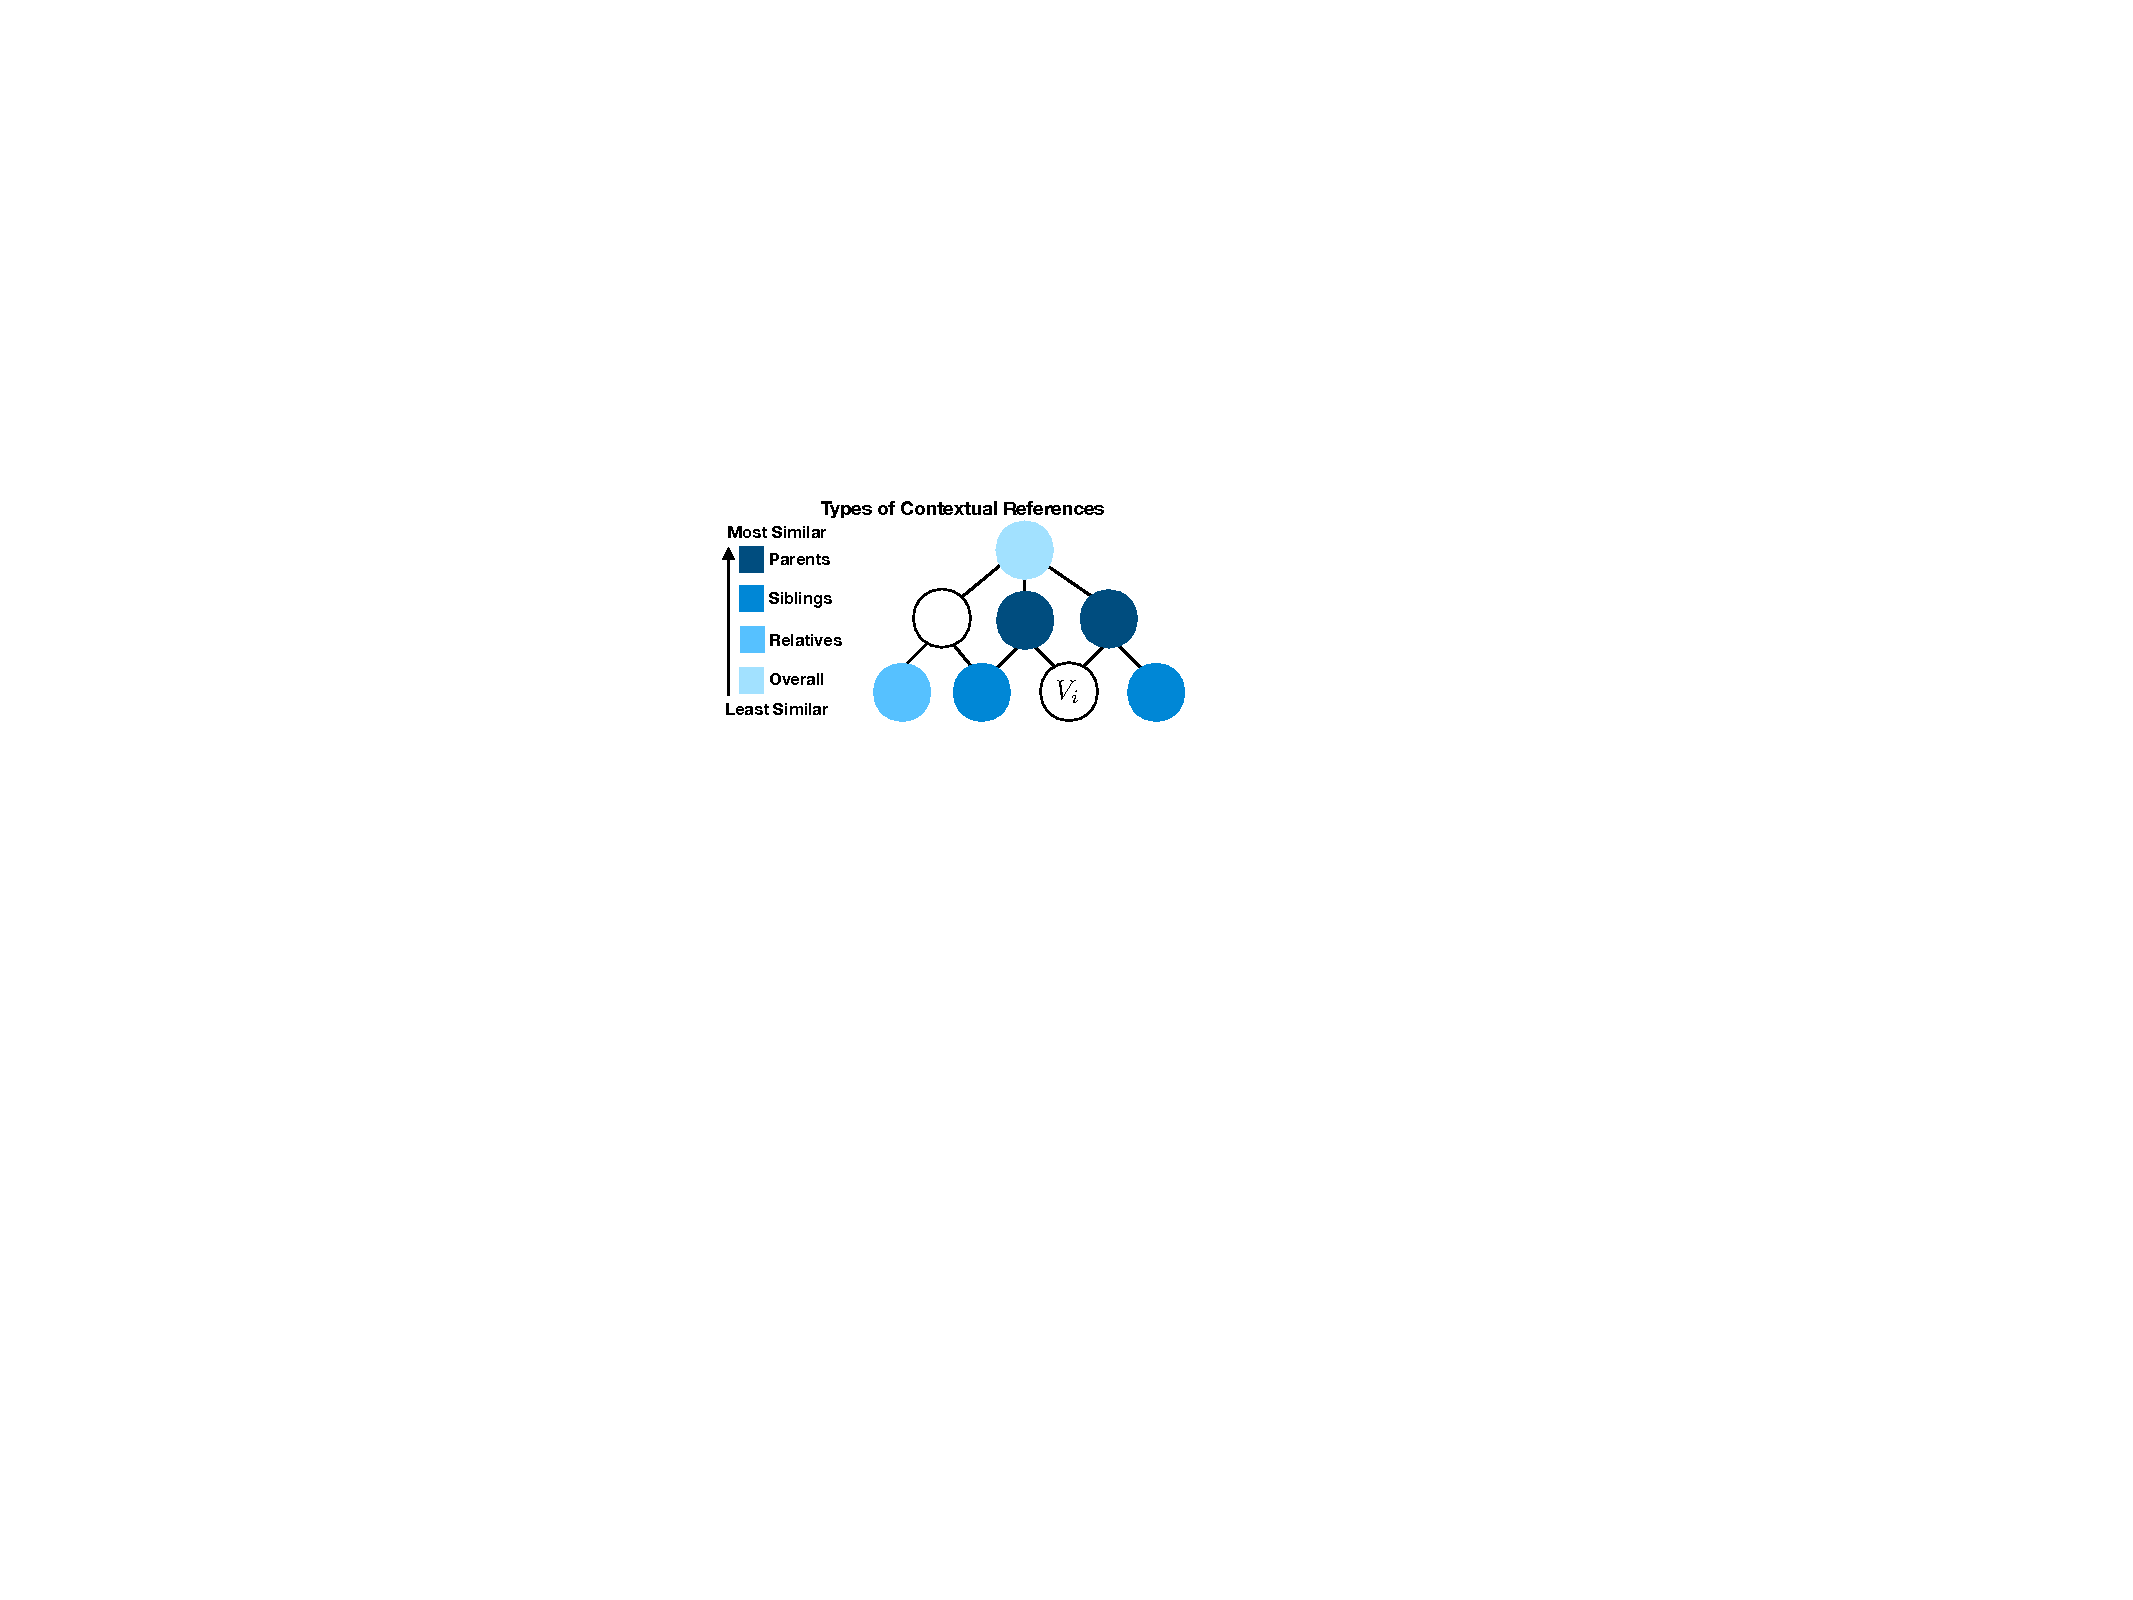
\includegraphics[width=0.7\linewidth]{figures/contextual_reference.pdf}
\caption{\change{Different types of contextual references} for a given visualization of interest $V_i$. The degree of similarity with respect to $V_i$ is denoted by darkest to lightest color hue.\agp{I don't see how the relative is actually a relative. It shares no similarity with $V_i$, and is no different from the other white node. (One way to see this is that the common ancestor for both the so-called relative and the white node and $V_i$ are the same -- the overall one.)}}
\label{fig:reference}
\vspace{-10pt}
\end{figure}
\par \change{Studying participants' use of contextual references reveals inherent challenges that arise from using the dashboards generated by \BFS and \cluster.} For \cluster, participants mainly compared against relatives and overall visualizations. Since \cluster optimizes the diversity of shape distributions amongst the visualizations, the selected visualizations had up to 4 filters and were disconnected from each other. For this reason, in many cases\change{,} participants could only rely on relatives and the overall visualizations as contextual references. For example, P4.A2 pointed at a 4-filter visualization with extreme values (100\% for warning; 0\% for arrest and ticket) and indicated how ``\textit{a lot of [the visualizations] are far too specific. This is not very helpful. You can't really hypothesize that all people are \change{[sic]} going to be warned, because it is such a specific category, it might just be one person}''. %, you need to have a bigger dataset. And that category will not really give you such extremes to make it more credible''.
He further explained how he ``\textit{would not want to see the intersections [(visualizations with many filters)] at first and would want to see all the bases [(univariate summaries)] then dig in from there.}'' The lack of informative contextual references in the \cluster dashboard is also reflected in how analysts exhibited high variance and deviation in their prediction responses. Note that the prediction task was chosen so that exactly one parent must be present in the dashboard, so these results do not point to the absence of parent visualizations in these \change{dashboards}, but rather indicate how participants made use of the information presented in the dashboards to form their prediction.
\par Furthermore, \change{improper comparisons against contextual references often make} it difficult for analysts to \change{interpret} displayed visualizations. In particular, when visualizations composed of multiple filter conditions were shown in \cluster dashboards, 25\% of participants had trouble \change{making sense of the meaning of a filter} for at least one of the datasets \change{(e.g., understanding that \texttt{gender=F AND age=60+} corresponds to female drivers with ages larger than 60 years old) at some point during the study}. In contrast, as shown in Table~\ref{table:thematic_summary}, this confusion only happened once for \BFS and none for \system. This is due to the fact that \cluster dashboards \change{seemed} random to the users, making it challenging to find ``close'' contextual references to compare against and form an accurate mental model. \change{In contrast, the linear ordering of \BFS and hierarchical ordering of \system were natural and interpretable for participants}. %In contrast, \BFS follows a linear ordering and \system follows a hierarchical ordering, which were more natural and interpretable for participants.
%despite our modification to KMeans which picks the visualizations with the least number of filters to show in the dashboard for improving interpretability
%These themes are drawn from user's explanations of how they obtained certain insights or ---- that --different tasks or while interpreting the dashboards. 4 categories :
\par For \BFS, most comparisons were based on the overall and siblings. Due to the sequential level-wise picking approach, the overall visualization for \BFS dashboards corresponded to the immediate parent, so they are not explicitly recorded as a parent. While the overall and sibling comparisons can be informative, \change{the incomplete comparisons, due to the limited number of first-level visualizations displayed, can result in flawed reasoning, likewise observed in the aforementioned Autism prediction task.} In contrast, for \system, almost all users compared against the overall and parents, while some also exploited \change{sibling comparisons} to make weaker guesses for less-frequently observed attributes (e.g., using a 2-filter sibling visualization involving \texttt{driver\_age} to infer another 2-filter visualization involving \texttt{driver\_age} with a different parent.)
% \subsection{Improper contextual reference can lead to misleading insights.}
\begin{table*}[ht!]
	\centering
	\begin{tabular}{|l|l|l|l|}
	\hline & \system & \cluster & \BFS \\ \hline
	Difficulty with Interpreting Visualizations & 0 & \cellcolor[HTML]{FD6864}3 & 1 \\ \hline
	Misjudged Significance of Potential Small-Size Population & 0 & \cellcolor[HTML]{FD6864}4 & 1 \\ \hline
	Interpretable ``Human-like" Dashboard & \cellcolor[HTML]{9AFF99}5 & 1 & 0 \\ \hline
	Number of Insights (Police) & \cellcolor[HTML]{9AFF99}11 & 8 & 9 \\ \hline
	Number of Insights (Autism) & \cellcolor[HTML]{9AFF99}16 & 6 & 11 \\\hline
	\end{tabular}
\caption{Summary of qualitative insights from thematic coding. We record the total number of insights based on overall \change{dataset findings} that \change{were} independently discovered by more than two different participants. For each participant, we coded the absence or presence of 7 such insights for the Police dataset and 6 insights for the Autism dataset.}%findings regarding the dataset or information regarding one or more attributes
\label{table:thematic_summary}
\vspace{-15pt}
\end{table*}
% \subsection{The Danger of Improper References}%, echoing our previous concern regarding the danger of small subpopulation sizes. This issue stems from the fact that the contextual reference used for comparison was the overall population, however the unseen parent subpopulation may have behaved very differently.
\tr{
	\subsection{The Danger of Small Subpopulations}
	The danger of spurious patterns and correlations in visualizations that contain small subpopulation size is a well-known problem in exploratory analysis~\cite{Binnig2017}. When examining visualizations with many filters and extremely-skewed values in one or more bars (bars with 100\% or 0\%), 4 \cluster participants did not realize that charts with multiple filters may have a smaller subpopulation size. In contrast, 6 of the participants using \system explicitly noted that while these extreme-valued visualizations may be interesting, they were less certain due to the unknown subpopulation size and should be investigated further. For example, P1.A1 noted that a visualization with warning=100\% caught her eye, ``\textit{but I don't know what the N is, maybe it's one person, this makes me a little skeptical, that makes me want to go back to the raw data and look at what is the N and what drives something so drastic?}'' We also found that this subpopulation-size fallacy was observed to be more severe for the Autism dataset, where participants had less intuition on the expected attribute behavior.  Since \BFS dashboards only displayed first-level visualizations, participants for \BFS did not see visualizations with large numbers of filters that had small subpopulations during the study, so none of the \BFS participants exhibited signs of this fallacy.
}
% \subsection{Hierarchical layout leads to more natural contextual comparisons compared to table layout.}
%it was easier to follow contextual references in \system
\subsection{Interpretability of Hierarchical Layouts}
\par In the post-study interviews, participants cited hierarchical layout as \change{a} key reason \change{for why they preferred \system recommendations}. \change{Even though participants were never explicitly told what the edge connections between the visualizations meant during the study, they were able to interpret the meaning of the dashboards effortlessly through \system's hierarchical layout}. For example, P1.A1 stated that ``\textit{the hierarchical nature [is] a very natural flow...so when you are comparing, you don't have to be making those comparisons in your head, visually that is very pleasing and easy to follow.}'' %Likewise, [P8.A1] also stated that ``I like the different levels, it makes it very visually easy to figure out what you want to look at, if you want to look at the overall data, it's right there at the top for you, if you want to get more specific, you just follow a branch downwards, which I think is very intuitive.''
Likewise, P9 described how \system's hierarchical layout for the Autism dataset was a lot easier to follow than the Police dataset shown in the table layout for \cluster:
\begin{quote}
\textit{If I had to look at this dataset in the format of the other one, this would be much more difficult. It was pretty hard for me to tell in the other one how to organize the tree, if there was even a tree to be organized. I like this layout much better, I think this layout allows me to approach it in a more meaningful way. I can decide, what do I think matters more: the overall trend? or the super detailed trends? and I know where to look to start, in the other one, every time I go back to it, I would say, where's the top level, where's the second level? I mentally did this. Like when you asked me that first question, it took much longer to find it, because I literally have to put every chart in a space in my head and that took a lot longer than knowing how to look at it.}
\end{quote}
At the end of the study, some participants \change{who were assigned dashboard conditions with table layouts} sketched and explained how they would like the layout of the visualizations to be done. \change{These} participants expressed that they wanted ``groupings'' or layouts that arranged visualizations with the same attribute together. Other participants advocated for isolating the overall visualization outside of the dashboard table for facilitating easier comparisons. Both of these suggestions provide further motivation for our hierarchical organization of visualizations. \change{\papertext{Our findings echo prior work on visualization sequences and storytelling~\cite{Hullman2017,Segel2010,Boy2015,Kim2017}, which found that analysts prefer visualization sequences structured hierarchically based on shared data properties such as levels of aggregation ordered by increasing levels of summarization.}}
%Kim et al.~\cite{Kim2017} modeled relationships between charts by empirically estimating transition (edge) cost between moving from one visualization (node) to another. They found that participants preferred ``\textit{starting from the entire data and introducing increasing levels of summarization}''.
 %layout and the idea of the collapsed visualizations as described earlier.%in Section \ref{sec:interaction}.
\par Since we did not inform participants about how the dashboards were generated, it was \change{surprising to see} that some participants \change{presumed} that the dashboards were hand-picked by a human analyst and \change{hypothesized} what this \change{fictitious analyst}'s intentions were (e.g., ``\textit{It seems like the researcher who created this dashboard was specifically looking at people of Asian descent and people who are 60 or older.}'' [P7.A1]). \change{Table~\ref{table:thematic_summary} shows how} 5 out of 12 participants referred to the \system dashboards as if they were generated by a human, whereas there was only 1 participant for \cluster and none for \BFS made such remarks\change{\footnote{We encoded this phenomenon by looking at instances where a participant either explicitly \change{referred} to a person who picked out the dashboard or implicitly described their intentions through personal pronouns.}}. At the end of the study, many were surprised to learn that the \system dashboard was actually picked out by an algorithm, indicating that \system could automatically \change{generate convincing dashboards similar to ones that were} authored with human intention. The interpretability of \system dashboards may have contributed to the increased number of insights discovered in both datasets compared to the two baselines, as summarized in Table~\ref{table:thematic_summary}.
\stitle{Limitations of \system}
% Interestingness task is highly subjective, so not conclusive whether interesting or not , despite the positive result
% Due to the highly subjective nature of the retrieval task, the interestingness selection for the Police dataset was biased by participant's priors and intuition about the attributes. For example, while all participants who have seen the visualization "duration=30+min" verbally noted that stop duration is a crucial factor that leads to arrest, only 4 users marked it as interesting. 5 participants marked the visualization as not interesting and 4 left it unselected, because the visualization was not very surprising as it agreed with their intuition that ``\textit{if the police stop is taking a long time, something has probably gone wrong}''.
\par As described earlier, since the details of how the dashboards were obtained \change{were} not explained to the users during the study, some users expressed that they were initially confused by \system \change{as} not all variables were present in the dashboard. Others also found it confusing that the addition of filters did not always correspond to the same variables. For example, P2.A1 criticized how the dashboard was intentionally selected to be biased:
\begin{quote}
\textit{I feel like this one, not all the data is here, so we are already telling a story, you are trying to steer the viewer to look at certain things. And the focus seems to be on where the arrest rate is high. You probably could have found other things that led to ticket being high, but you didn't pull those out. You are trying to see if there are other factors that lead to more arrests.}
\end{quote}
\npar This sentiment is related to participants' desire to perform their own ad-hoc querying alongside the dashboard to inspect other related visualizations for verifying their hypothesis. For example, P7.A1 wanted to inspect all other first-level visualizations for driver's race to assess its influence. P7.A1 expressed that while he had learned many insights from the dashboard, ``\textit{the only thing I don't like is I cannot control the types of filter, which is fixed.}'' \change{Since the design objective for \system is to support and evaluate its capability to provide informative dashboards, \system is limited in its interactivity and the extent of free-formed data exploration it supports. This result also points to how} \system could serve as a helpful \change{assistant} alongside other conventional visualization tools, such as Tableau. Outside the context of the user study, it is essential to explain how \system \change{selects} the visualizations in \change{an} easy and interpretable manner to establish a sense of summarization guarantee for the users and help them make better inferences with the dashboard.

\change{%a small set of analytic tasks corresponding to each design objectives, with
	\par Since the goal of our study is to evaluate whether \system can assist users in drill-down exploration, our preliminary study is limited to comparison against baselines stemming from conventional approaches for multidimensional data exploration. While we understand how the \system study condition may confound both the hierarchical layout with the algorithmic choice of visualizations, our intention for the baseline was to simulate how analysts generate a large number of visualizations individually, typically arranged in a table grid layout, rather than using a hierarchical layout. Further evaluation comparing how the different hierarchically-displayed visualization selection algorithms assist users in drill-down exploration is a direction of future work.
}
\tr{
	\par As discussed earlier, subpopulation size is important in establishing the significance of a trend observed in a visualization. While subpopulation size is taken into account implicitly in our objective, we should design interfaces that convey the notion of subpopulation size in our dashboard. Examples include Sankey-like flow diagrams indicating the percentage of the parent population broken down into individual subpopulations and subpopulation size explicitly specified via edge labels.
}


%, either explicitly displayed as text when hovering over the visualization or changing the size or background color of the visualizations to encode subpopulation size.
%“I actually found it really confused at first because such a low arrest rate at the top, and then at the bottom the arrest rate was much higher, so I was like is this data wrong. Then I realized we’re not looking at all the data here, you’ve pulled out some of it. It took me a minute to realize that. And once I read the title of the charts I realized that makes sense.” [P2.A1]
% - Reference of Comparison
% - Layout naturally lends itself for comparison:
% 	- describe ordering layout, how participants naturally follow the flow
% 	- emph that we did not tell them what the edge connections mean and how they were computed but the users naturally figured it out, that it means adding an additional filter.
% 	- hierarchical interpretable nature (quotes)
% 	- compared to other baselines
% 	- describe dashboard by human (count)
% - Misleading insights v.s. True insight discovery rates
% 	- Interpretability:
% 	- misled understanding subpopulation size
% 		- for autism, it is important to see if they compare to overall because if not they would think high skew to NO is important whereas its actually pretty close to overall.
% 	- trouble interpreting filter combination
%%%%%%%%%%%%%%%%%%%%%%%%%%%%%%%%%%%%%%%%%%%%%%%%%%%%%%%%%%%%%%%%%%%%%%%%%%%%%%%%%%%%%%%%%%%%%%%%%%%%%%%%%%%%%%%%%%%%%%%%
%%%%%%%%%%%%%%%%%%%%%%%%%%%%%%%%%%%%%%%%%%%%%%%%%%%%%%%%%%%%%%%%%%%%%%%%%%%%%%%%%%%%%%%%%%%%%%%%%%%%%%%%%%%%%%%%%%%%%%%%
%%%%%%%%%%%%%%%%%%%%%%%%%%%%%%%%%%%%%%%%%%%%%%%%%%%%%%%%%%%%%%%%%%%%%%%%%%%%%%%%%%%%%%%%%%%%%%%%%%%%%%%%%%%%%%%%%%%%%%%%
% \subsection{Statistical Paradoxes}\dor{make title full sentences}
% Visualizations are powerful representations for studying different distributions or patterns in a dataset, but our human intuition could often mislead us when it comes to interpreting those patterns\cite{Binnig2017,Wall2017}. Several statistical paradoxes can lead analysts to draw incorrect conclusions from observed visualizations, including Simpson's paradox as discussed in the introduction. The key reason why many of these paradoxes emerge is the \emph{incompleteness} of the observed data or lack of focus on relevant informative subsets of the data. For example, Simpson's paradox arises in the presence of an unseen confounding variable. %likewise, the absence of  base rate information causes base rate fallacy.
%  We assert \dor{too strong of a sentence} that distributional awareness can be useful in avoiding such statistical paradoxes. If an analyst is aware of all distributions in a given dataset, he/she is less prone to many statistical paradoxes. However, given the large number of dimensions and high cardinality of these dimension in modern datasets, it is not possible for an analyst to explore and memorize all distributions. Therefore, a more evolved approach is to be aware of the exceptional distributions. In this work, we propose a first step towards this goal, where we identify the exceptional distributions in terms of their informative references. The remaining (unseen) distributions in the dataset are rather unsurprising and can be inferred from the visualizations in the dashboard. \dor{I would recommend first talk about issue with large dimension + danger of multiple hypothesis testing + incomplete testing, point out problem, then talk about how our system resolves this.}
% \subsection{Structural Insight}
% Our proposed dashboard consists of a hierarchy of visualizations, where each visualization is linked to its most informative parent. The shape or structure of the hierarchy contains useful information that augments the information learned from the visualizations and aid distribution awareness and understanding. \dor{what's interesting here is that while many work have looked at visualization presentation, layout of presentation never considered, we find in Sec 5 that this is actually important and can encode info.} For example, the depth and branching factor of the hierarchy could inform a user regarding the configuration of insights. Deep hierarchies contain long paths, i.e., insights are present at lower level visualizations with multiple constraints. In contrast, bushy hierarchies (with high branching factor) contain cases where multiple visualizations have the same informative parent and they differ from that parent. \dor{do we have examples from the study that support this?} We assert that the depth and branching factor could be a meaningful constraint in our problem formulation \dor{too strong of a sentence}. Some applications for example, funnel exploration require studying deep hierarchies, whereas others for example, building decision trees require studying bushy hierarchies. A natural extension of our current problem formulation is to allow users to select the depth and branching factor for the hierarchy.
% \subsection{Other Visualization Lattices}
% In this work, we explore the space of data subsets to generate our visualization lattice. Note that it is possible to explore the space of dimension attributes in x-axis to generate a different visualization lattice. In particular, given a combination of dimension attributes $X = \{X_1, \ldots, X_n\}$, adding one or more new dimensions in $X$ will generate a new combination. An ancestor-descendant relationship exists between these dimension combinations, following the same principles of Section 3.1. These relationships lead to a new lattice, which we call the dimension combination lattice. Our informative deviation based approach could be used for traversing the dimension combination lattice. However, we observe that most users do not visualize more than two attributes in x-axis. Therefore, traversing the dimension combination lattice is not very useful for most applications.
% \dor{I think 6.2,6.3 don't tie well with the rest of the paper. It sounds like stretching our own ideas rather than being motivated by the work done in this paper. Other potentially more relevant discussion: distribution awareness and how it might be useful in other contexts? Decision trees?}
% %\subsection{Utility Metrics}

%!TEX root = main.tex
\section{Conclusion}
\par Common analytics tasks, such as causal inference, feature selection, and outlier detection require studying data distributions at different levels of data granularity~\cite{Anand2015,Wu2013,Heer2012}. However, without knowing \textit{what} subset of data contains an insightful distribution, manually exploring distributions from all possible data subsets can be tedious and inefficient. Moreover, when examining data subsets by adding one filter at a time, analysts can fall prey to the drill-down fallacy, where they mistakenly attribute the interestingness of a visualization to a ``local difference'', while overlooking a more general explanation for the root cause of the behavior. To address these issues, we presented \system, an interactive visualization recommendation system that automatically selects a small set of informative and interesting visualizations to summarize the distributions within a dataset. Our user study results demonstrate that our tool can guide analysts towards more informed decisions for retrieving interesting visualizations, judging the relative importance of attributes, and predicting unseen visualizations, than compared to the two other summarization baselines. Study participants also find dashboard generated by \system to be more interpretable and ``human-like'', leading to more discovered insights. Our work is one of the first automated systems that guides analysts across the space of data subsets by summarizing key insights with safety guarantees---a step towards our grander vision of developing intelligent tools for accelerating and assisting with visual data discovery.  
% discovery 
% - Drill down is hard and dangerous
% - Drill down fallacy
% - In this paper, we develop ----
% - \system does X, Y , Z
% Our user study shows that ----\system compared to baselines
% 	- perform better in a wide range of analytic task such as attribute ranking, prediction, and interestingness. 
% 	- interpretable, more insights
% - Wider implications
% \bibliographystyle{abbrv}
\bibliographystyle{abbrv-doi}
\bibliography{reference}

\end{document}
